% !TEX encoding = UTF-8 Unicode
%DIF LATEXDIFF DIFFERENCE FILE
%DIF DEL discussion_paper.tex      Sat Jun  1 11:54:45 2019
%DIF ADD landscape_evolution.tex   Sat Jun  1 11:13:54 2019

% Geoscientific Model Development (gmd)
\documentclass[gmd, manuscript]{copernicus}

% packages
\usepackage{tabu}
\usepackage{booktabs}
\usepackage{graphicx}
\usepackage[export]{adjustbox}
\usepackage[utf8]{inputenc}
\usepackage{listings}
\usepackage[percent]{overpic}
%DIF PREAMBLE EXTENSION ADDED BY LATEXDIFF
%DIF CTRADITIONAL PREAMBLE %DIF PREAMBLE
\RequirePackage{color}\definecolor{RED}{rgb}{1,0,0}\definecolor{BLUE}{rgb}{0,0,1} %DIF PREAMBLE
\RequirePackage[stable]{footmisc} %DIF PREAMBLE
\providecommand{\DIFadd}[1]{{\protect\color{blue} \sf #1}} %DIF PREAMBLE
\providecommand{\DIFdel}[1]{{\protect\color{red} [..\footnote{removed: #1} ]}} %DIF PREAMBLE
%DIF SAFE PREAMBLE %DIF PREAMBLE
\providecommand{\DIFaddbegin}{} %DIF PREAMBLE
\providecommand{\DIFaddend}{} %DIF PREAMBLE
\providecommand{\DIFdelbegin}{} %DIF PREAMBLE
\providecommand{\DIFdelend}{} %DIF PREAMBLE
%DIF FLOATSAFE PREAMBLE %DIF PREAMBLE
\providecommand{\DIFaddFL}[1]{\DIFadd{#1}} %DIF PREAMBLE
\providecommand{\DIFdelFL}[1]{\DIFdel{#1}} %DIF PREAMBLE
\providecommand{\DIFaddbeginFL}{} %DIF PREAMBLE
\providecommand{\DIFaddendFL}{} %DIF PREAMBLE
\providecommand{\DIFdelbeginFL}{} %DIF PREAMBLE
\providecommand{\DIFdelendFL}{} %DIF PREAMBLE
%DIF END PREAMBLE EXTENSION ADDED BY LATEXDIFF

\begin{document}

%DIF > \title{\lowercase{r.sim.terrain 1.0}: a dynamic landscape evolution model} 
\title{\DIFdelbegin %DIFDELCMD < \lowercase{r.sim.terrain}%%%
\DIFdelend \DIFaddbegin \lowercase{r.sim.terrain 1.0}\DIFaddend : a \DIFdelbegin \DIFdel{dynamic }\DIFdelend landscape evolution model \DIFaddbegin \DIFadd{with dynamic hydrology}\DIFaddend } 

\Author[1]{Brendan Alexander}{Harmon}
\Author[2,3]{Helena}{Mitasova}
\Author[2,3]{Anna}{Petrasova}
\Author[2,3]{Vaclav}{Petras}

\affil[1]{Robert Reich School of Landscape Architecture, Louisiana State University, Baton Rouge, Louisiana, USA}
\affil[2]{Center for Geospatial Analytics, North Carolina State University, Raleigh, North Carolina, USA}
\affil[3]{Department of Marine, Earth, and Atmospheric Sciences, North Carolina State University, Raleigh, North Carolina, USA}

\DIFdelbegin %DIFDELCMD < \runningtitle{\lowercase{r.sim.terrain}: a dynamic landscape evolution model}
%DIFDELCMD < %%%
\DIFdelend \DIFaddbegin \runningtitle{\lowercase{r.sim.terrain 1.0}: a landscape evolution model with dynamic hydrology} 
\DIFaddend 

\runningauthor{Brendan Harmon}

\correspondence{Brendan Harmon (baharmon@lsu.edu)}

\received{}
\pubdiscuss{}
\revised{}
\accepted{}
\published{}

\firstpage{1}

\maketitle

\begin{abstract}
While there are numerical landscape evolution models
that simulate how steady state flows of water and sediment
reshape topography over long periods of time, 
r.sim.terrain is the first to 
simulate short-term topographic change 
for both steady state and dynamic flow regimes
across a range of spatial scales.
This free and open source, 
GIS-based topographic evolution model
uses empirical models for soil erosion
\DIFdelbegin \DIFdel{at watershed to regional scales 
}\DIFdelend and a physics-based model
for shallow overland water flow and soil erosion 
\DIFdelbegin \DIFdel{at subwatershed scales
}\DIFdelend to compute short-term topographic change. 
This \DIFdelbegin \DIFdel{either }\DIFdelend \DIFaddbegin \DIFadd{model uses either a }\DIFaddend steady state or dynamic \DIFdelbegin \DIFdel{model simulates
}\DIFdelend \DIFaddbegin \DIFadd{representation of overland flow
to simulate }\DIFaddend how overland sediment mass flows reshape topography
for a range of hydrologic soil erosion regimes
based on topographic, land cover, soil, and rainfall parameters. 
As demonstrated by a case study 
for Patterson Branch subwatershed
on the Fort Bragg military installation in North Carolina,
r.sim.terrain \DIFdelbegin \DIFdel{can realistically simulate }\DIFdelend \DIFaddbegin \DIFadd{simulates }\DIFaddend the development of 
fine-scale morphological features including 
ephemeral gullies, rills, and hillslopes.
Applications include land management, erosion control,
landscape planning, and landscape restoration. 
\end{abstract}

\copyrightstatement{...}

% --------- INTRO FIGURE ---------

\begin{figure}%[H]
\center
\includegraphics[width=\textwidth,height=0.925\textheight,keepaspectratio]{figures/evolution.pdf}
\caption{
The digital elevation model (DEM) 
\DIFdelbeginFL \DIFdelFL{before }\DIFdelendFL (a\DIFdelbeginFL \DIFdelFL{.}\DIFdelendFL ) \DIFaddbeginFL \DIFaddFL{before }\DIFaddendFL and \DIFdelbeginFL \DIFdelFL{after }\DIFdelendFL (b\DIFdelbeginFL \DIFdelFL{.}\DIFdelendFL ) \DIFaddbeginFL \DIFaddFL{after
}\DIFaddendFL simulated landscape evolution with r.sim.terrain 
\DIFaddbeginFL \DIFaddFL{for a subwatershed of Patterson Branch, Fort Bragg, NC, USA}\DIFaddendFL . 
\DIFaddbeginFL \DIFaddFL{(a) The before DEM was generated from an airborne lidar survey in 2012. 
}\DIFaddendFL This simulation used the SIMWE model
for a 120~\unit{min} rainfall event with \DIFdelbeginFL \DIFdelFL{25}\DIFdelendFL \DIFaddbeginFL \DIFaddFL{50}\DIFaddendFL ~\unit{mm~hr}$^{-1}$
\DIFdelbeginFL \DIFdelFL{in }\DIFdelendFL \DIFaddbeginFL \DIFaddFL{for }\DIFaddendFL a \DIFdelbeginFL \DIFdelFL{transport limited soil erosion }\DIFdelendFL \DIFaddbeginFL \DIFaddFL{variable erosion-deposition }\DIFaddendFL regime at steady state.
\DIFaddbeginFL \DIFaddFL{(b) }\DIFaddendFL In the evolved DEM 
\DIFdelbeginFL \DIFdelFL{(b.)
}\DIFdelendFL the gully channel has widened 
with depositional ridges forming along its thalweg.}
\label{fig:evolution}
\end{figure}

% --------- BODY ---------

\introduction
Landscape evolution models represent how the surface of the earth changes 
over time in response to physical processes. 
Most studies of landscape evolution have been descriptive, 
but a number of numerical landscape evolution models 
have been developed that simulate elevational change over time 
\DIFdelbegin \DIFdel{\citep{Temme2013}}\DIFdelend \DIFaddbegin \DIFadd{\citep{Tucker2010,Temme2013}}\DIFaddend . 
% numerical models
Numerical landscape evolution models
such as the Channel-Hillslope Integrated Landscape Development (CHILD) model 
\citep{Tucker2001}\DIFdelbegin \DIFdel{and SIBERIA \citep{Willgoose2005}}\DIFdelend \DIFaddbegin \DIFadd{,
CAESAR \citep{Coulthard2002,Coulthard2012},
SIBERIA \citep{Willgoose2005},
LAPSUS \citep{Schoorl2000,Schoorl2002},
and r.landscape.evol \citep{Barton2010}
}\DIFaddend simulate steady state flows over long temporal scales.
% recent development
\href{http://landlab.github.io/}{Landlab},
a new Python library for numerically modeling Earth surface processes
\citep{Hobley2017},
has components for simulating landscape evolution such as the 
Stream Power with Alluvium Conservation and Entrainment (SPACE) 
model \citep{Shobe2017}.
% gis-based models
While Geographic Information Systems (GIS)
support efficient data management, 
spatial and statistical modeling and analysis, 
and visualization,
there are few GIS-based soil erosion models \DIFaddbegin \DIFadd{(see Table~\ref{table:erosion_models})
}\DIFaddend or landscape evolution models\DIFdelbegin \DIFdel{(see Tables~\ref{table:erosion_models}-\ref{table:evolution_models}) }\DIFdelend \DIFaddbegin \DIFadd{.
%DIF >  r.terradyn
\cite{Thaxton2004} developed the model r.terradyn as a GRASS GIS shell script module 
to simulate terrain evolution by steady-state net erosion deposition rates
estimated by the Simulation of Water Erosion (SIMWE) model \citep{Mitas1998}
and gravitational diffusion. 
%DIF >  r.landscape.evol
\cite{Barton2010} developed a long term landscape evolution model
in GRASS GIS called r.landscape.evol that integrates 
the Unit Stream Power Erosion Deposition (USPED) model,
fluvial erosion, and gravitational diffusion.
r.landscape.evol has been used to simulate the impact 
of prehistoric settlements on Mediterranean landscapes}\DIFaddend .
% research questions
\DIFdelbegin \DIFdel{Furthermore there }\DIFdelend \DIFaddbegin \DIFadd{There }\DIFaddend are still major research questions 
to address in the theoretical foundations of erosion modeling 
such as how erosional processes scale over time and space 
and how sediment detachment and transport interact \citep{Mitasova2013}. 
% dynamic evolution
While most numerical landscape evolution models 
simulate peak flows at steady state\DIFdelbegin \DIFdel{(see Table~\ref{table:evolution_models})}\DIFdelend ,
short-term erosional processes like gully formation can be dynamic
with significant morphological changes happening within minutes
before flows reach steady state. 
A \DIFdelbegin \DIFdel{dynamic }\DIFdelend landscape evolution model \DIFaddbegin \DIFadd{with dynamic water and sediment flow
}\DIFaddend is needed to study fine-scale spatial and short-term temporal erosional processes
such as gully formation and the development of microtopography. 

% steady state versus dynamic
At the beginning of a rainfall event 
the overland water flow \DIFdelbegin \DIFdel{regime is dynamic }\DIFdelend \DIFaddbegin \DIFadd{is unsteady }\DIFaddend -- 
its depth changes at a variable rate over time and space. 
If the intensity of rainfall continues to change throughout the event
then the flow regime will remain dynamic. 
% steady state
If, however, the overland flow reaches a peak rate
then the hydrologic regime is considered to be at steady state.
At steady state:
% steady state eq.
\begin{equation}
\label{eq:steady_state}
{\partial h(x,y,t) \over \partial t} = 0
\end{equation}
%
{\small
\noindent
where: \\
\noindent
\hspace*{0.5em} $(x,y)$ is the position [\unit{m}]\\
\hspace*{0.5em} $t$ is the time [\unit{s}]\\
\hspace*{0.5em} $h(x,y,t)$ is the depth of overland flow [\unit{m}]\\
}

% gully formation
Gullies are eroded, steep banked channels 
formed by ephemeral, concentrated flows of water.
A gully forms when overland waterflow
converges in a knickzone
-- a concave space with steeper slopes than its surroundings 
\citep{Zahra2017} -- 
during intense rainfall events.  
When the force of the water flow concentrated in the knickzone
is enough to detach and transport large amounts of sediment,
an incision begins to form at the apex of the knickzone 
-- the knickpoint or headwall.
As erosion continues the knickpoint begins to migrate upslope
and the nascent gully channel widens,
forming steep channel banks. 
Multiple incisions initiated by different knickpoints 
may merge into a gully channel
and multiple channels may merge 
into a branching gully system \citep{Mitasova2013}. 
%DIF >  detachment limited
This erosive process is dynamic; 
the morphological changes drive further changes 
in a positive feedback loop\DIFdelbegin \DIFdel{until water flow reaches steady state}\DIFdelend .
When the gully initially forms 
the soil erosion regime should be detachment capacity limited
with the concentrated flow of water in the channel of the gully 
detaching large amounts of sediment 
and transporting it to the foot of the gully, 
potentially forming a depositional fan.
\DIFdelbegin \DIFdel{After the initial formation of the gully
}\DIFdelend %DIF >  variable erosion-deposition
\DIFaddbegin \DIFadd{If the intensity of rainfall decreases
and transport and detachment capacity 
approach a balance, 
then }\DIFaddend the soil erosion regime may switch to 
\DIFaddbegin \DIFadd{a variable }\DIFaddend erosion-deposition \DIFdelbegin \DIFdel{if the intensity of rainfall decreases}\DIFdelend \DIFaddbegin \DIFadd{regime,
in which soil is eroded and deposited 
in a spatially variable pattern}\DIFaddend .
Subsequent rainfall events may trigger further 
knickpoint formation and upslope migration, 
channel incision and widening, and
depositional fan and ridge formation. 
Between high intensity rainfall events, 
lower intensity events and gravitational diffusion
may gradually smooth the shape of the gully. 
%DIF >  transport limited
Eventually, if detachment capacity 
significantly exceeds transport capacity
\DIFaddbegin \DIFadd{and the regime switches to transport capacity limited}\DIFaddend , 
the gully may fill with sediment\DIFaddbegin \DIFadd{,
as soil continues to be eroded, but is not transported far}\DIFaddend . 

% gully monitoring
Gully erosion rates and evolution
can be monitored in the field 
or modeled on the computer. 
% field methods
Field methods include
dendrogeomorphology \citep{Malik2008} and 
permanent monitoring stakes for recording erosion rates, 
extensometers for recording mass wasting events, 
weirs for recording water and suspended sediment discharge rates, 
and time series of surveys using 
total station theodolites \citep{Thomas2004},
unmanned aerial systems (UAS) \DIFaddbegin \DIFadd{\citep{Jeziorska2016,Kasprak2019,Yang2019}}\DIFaddend ,
airborne lidar \DIFaddbegin \DIFadd{\citep{Perroy2010,Starek2011}}\DIFaddend , 
and terrestrial lidar \DIFdelbegin \DIFdel{\citep{Starek2011,Bechet2016}}\DIFdelend \DIFaddbegin \DIFadd{\citep{Starek2011,Bechet2016,Goodwin2016,Telling2017}}\DIFaddend .
% high resolution topographic data
With terrestrial lidar, airborne lidar\DIFaddbegin \DIFadd{, }\DIFaddend and 
UAS photogrammetry
there is now sufficient resolution topographic data 
to morphometrically analyze and 
numerically model fine-scale landscape evolution in GIS
including processes such as gully formation 
and the development of microtopography. 
% gully simulation
Gully erosion has been simulated with 
\DIFdelbegin \DIFdel{the Revised Universal Soil Loss Equation Version 2 }\DIFdelend \DIFaddbegin \DIFadd{RUSLE2-Raster }\DIFaddend (RUSLER)
in conjunction with the Ephemeral Gully Erosion Estimator (EphGEE)
\citep{Dabney2014},
while gully evolution
has been simulated for detachment capacity limited erosion regimes
with the Simulation of Water Erosion (SIMWE) model
\citep{Koco2011, Mitasova2013}. 
Now numerical landscape evolution models 
that can simulate 
steady state and \DIFdelbegin \DIFdel{dynamic }\DIFdelend \DIFaddbegin \DIFadd{unsteady }\DIFaddend flow regimes
and \DIFdelbegin \DIFdel{can }\DIFdelend dynamically switch between soil erosion regimes 
are needed to study 
fine-scale spatial and short-term temporal erosional processes.

% aim
The numerical landscape evolution model 
r.sim.terrain was developed to 
simulate the spatiotemporal evolution of landforms
caused by shallow overland water and sediment flows
at spatial scales ranging from
square meters to kilometers
and temporal scales ranging from minutes to years. 
% objectives
This open source, GIS-based landscape evolution model can
simulate either steady state or \DIFdelbegin \DIFdel{dynamic }\DIFdelend \DIFaddbegin \DIFadd{unsteady }\DIFaddend flow regimes,
dynamically switch between soil erosion regimes, and
simulate the evolution of fine-scale morphological features 
such as ephemeral gullies
(Figure~\ref{fig:evolution}).
% questions
It was designed as a research tool for
studying how erosional processes scale over time and space,
comparing empirical and process-based models, 
comparing steady state and \DIFdelbegin \DIFdel{dynamic }\DIFdelend \DIFaddbegin \DIFadd{unsteady }\DIFaddend flow regimes, and
studying the role of \DIFdelbegin \DIFdel{dynamic }\DIFdelend \DIFaddbegin \DIFadd{unsteady }\DIFaddend flow regimes
in fine-scale morphological change. 
% testing
r.sim.terrain was tested with 
a subwatershed scale (450~\unit{m}$^{2}$) case study
and the simulations were compared against 
a time-series of airborne lidar surveys.

\section{r.sim.terrain}
\DIFaddbegin 

%DIF >  --------- CONCEPT MODEL ---------

\begin{figure}%DIF > [H]
\center
\includegraphics[width=\textwidth,keepaspectratio]{figures/concept.pdf}
\caption{\DIFaddFL{Conceptual diagram for r.sim.terrain.}}
\label{fig:evolution}
\end{figure}

%DIF >  ---------------------------------

\DIFaddend The process-based, spatially distributed 
landscape evolution model r.sim.terrain
simulates topographic changes
caused by shallow, overland water flow
across a range of spatiotemporal scales and soil erosion regimes
using either
the Simulated Water Erosion (SIMWE) model, 
the 3-Dimensional Revised Universal Soil Loss Equation (RUSLE 3D) model,
or the Unit Stream Power Erosion Deposition (USPED) model.  
\DIFaddbegin \DIFadd{The r.sim.terrain model
can simulate either steady state or dynamic flow regimes.
}\DIFaddend % simwe
SIMWE is a physics-based simulation
that uses a Monte Carlo path sampling method
to solve the water and sediment flow equations
for detachment limited, transport limited, and variable erosion-deposition 
soil erosion regimes 
\DIFdelbegin \DIFdel{\citep{Mitasova2004}}\DIFdelend \DIFaddbegin \DIFadd{\citep{Mitas1998,Mitasova2004}}\DIFaddend . 
With SIMWE 
r.sim.terrain
uses the modeled flow of sediment 
-- a function of water flow and soil detachment and transport parameters -- 
to estimate net erosion and deposition rates. 
% rusle3d
RUSLE3D is an empirical equation for \DIFdelbegin \DIFdel{sediment flows 
}\DIFdelend \DIFaddbegin \DIFadd{estimating soil erosion rates
}\DIFaddend in detachment capacity limited soil erosion regimes 
\DIFdelbegin \DIFdel{\citep{Mitasova1996}. 
}\DIFdelend \DIFaddbegin \DIFadd{\citep{Mitasova1996,Mitasova2013}. 
%DIF > 
}\DIFaddend With RUSLE3D r.sim.terrain
uses an event-based \DIFaddbegin \DIFadd{rainfall }\DIFaddend erosivity factor, 
\DIFdelbegin \DIFdel{the slope, the flow accumulation, and a }\DIFdelend \DIFaddbegin \DIFadd{soil erodibility factor, landcover factor, and }\DIFaddend 3D topographic factor
\DIFdelbegin \DIFdel{to model sediment flow}\DIFdelend \DIFaddbegin \DIFadd{-- a function of slope and flow accumulation --
to model soil erosion rates}\DIFaddend . 
% usped
USPED is \DIFdelbegin \DIFdel{an empirical }\DIFdelend \DIFaddbegin \DIFadd{a semi-empirical }\DIFaddend equation for net erosion and deposition 
in transport capacity limited soil erosion regimes 
\DIFaddbegin \DIFadd{\citep{Mitasova1996,Mitasova2013}}\DIFaddend . 
With USPED r.sim.terrain uses an event-based \DIFaddbegin \DIFadd{rainfall }\DIFaddend erosivity factor, 
\DIFdelbegin \DIFdel{the slope and aspect, the flow accumulation}\DIFdelend \DIFaddbegin \DIFadd{soil erodibility factor, landcover factor}\DIFaddend , and a 3D topographic factor
to model \DIFdelbegin \DIFdel{erosion-deposition as the the }\DIFdelend \DIFaddbegin \DIFadd{net erosion or deposition rates as the }\DIFaddend divergence of sediment flows. 
% evolution
For each of the models 
topographic change is derived at each time step
from the \DIFdelbegin \DIFdel{sediment flow or }\DIFdelend net erosion-deposition rate
and gravitational diffusion.
% regimes
\DIFdelbegin \DIFdel{The }\DIFdelend \DIFaddbegin \DIFadd{Depending on the input parameters, 
}\DIFaddend r.sim.terrain \DIFdelbegin \DIFdel{model
can simulate either steady state or dynamic flow regimes.
During }\DIFdelend simulations with SIMWE 
\DIFdelbegin \DIFdel{r.sim.terrain
can switch between 
detachment limited, transport limited, and variable }\DIFdelend \DIFaddbegin \DIFadd{can represent variable soil }\DIFaddend erosion-deposition \DIFdelbegin \DIFdel{soil erosion }\DIFdelend \DIFaddbegin \DIFadd{regimes, 
including prevailing detachment capacity limited 
or prevailing transport capacity limited }\DIFaddend regimes.

% capabilities
The r.sim.terrain model
can simulate the evolution of gullies
including processes such as 
knickpoint migration,
channel incision, 
channel widening, 
aggradation, and
scour pool and 
depositional ridge formation
along the thalweg of the gully. 
% applications
Applications include 
geomorphological research,
erosion control, 
landscape restoration, 
and scenario development 
for landscape planning and management.
% scale
This model can simulate landscape evolution 
over a wide range of spatial scales 
from small watersheds 
less than ten square kilometers
with SIMWE
to regional watersheds
of hundreds of square kilometers
with USPED or RULSE3D,
although it does not model fluvial processes. 
\DIFaddbegin \DIFadd{It has been used at resolutions ranging from sub-meter to 30~}\unit{m}\DIFadd{.
}\DIFaddend % implementation
\DIFdelbegin \DIFdel{This }\DIFdelend \DIFaddbegin \DIFadd{The }\DIFaddend model has been implemented 
as a Python add-on module 
for the free, open source
\href{https://grass.osgeo.org/}{Geographic Resources Analysis Support System (GRASS) GIS}
\citep{GRASS}. 
The source code is available at 
\url{https://github.com/baharmon/landscape\_evolution} 
under the GNU General Public License v2.
% parallel processing
It supports multithreading and parallel processing
to efficiently compute simulations 
using large, high resolution topographic datasets.
%
The landscape evolution model 
can be installed in GRASS GIS as an add-on module 
with the command: 
\begin{verbatim}
g.extension extension=r.sim.terrain
\end{verbatim}


% -------------------------- TABLE OF MODELS -----------------------------

\DIFaddbegin

% table of erosion models
\begin{table*}
\small
\caption{Geospatial soil erosion models}
\begin{tabu} to \textwidth {XXXXXl}
\toprule
Model & Spatial scale &  Temporal scale & Representation & Implementation & Reference\\
\midrule
RUSLE3D & regional & continuous & raster & map algebra & \citep{Mitasova1996}\\
USPED & watershed & continuous & raster & map algebra & \citep{Mitasova1996}\\
\href{https://grass.osgeo.org/grass74/manuals/r.sim.sediment.html}{SIMWE} & watershed & event -- & raster & \href{https://grass.osgeo.org/grass74/manuals/r.sim.sediment.html}{GRASS modules} & \citep{Mitas1998}\\
&& continuous\\
\href{http://geowepp.geog.buffalo.edu/}{GeoWEPP} & watershed & continuous & raster & \href{http://geowepp.geog.buffalo.edu/}{ArcGIS module} & \citep{Flanagan2013}\\
\href{https://www.tucson.ars.ag.gov/agwa/}{AGWA} & watershed & event -- & vector & \href{https://www.tucson.ars.ag.gov/agwa/}{ArcGIS module} & \citep{Guertin2015}\\
&& continuous\\
\href{https://blog.utwente.nl/lisem/}{openLISEM} & watershed & event & raster & \href{https://blog.utwente.nl/lisem/}{PCRaster script} & \citep{Roo1996}\\
\href{https://github.com/landlab/}{Landlab} & watershed & event -- & raster + mesh & \href{https://github.com/landlab/}{Python library} & \citep{Hobley2017}\\
&& continuous\\

\bottomrule
\\
\end{tabu}
\label{table:erosion_models}
\end{table*}
\DIFaddend

% <-------------------------------------------------------- CHECK DIFF HERE!

%DIF > % table of landscape evolution models
%DIF > \begin{table*}
%DIF > \small
%DIF > \caption{Topographic evolution models}
%DIF > \begin{tabu} to \textwidth {lXXXXll}
%DIF > \toprule
%DIF > Model &  Temporal scale & Representation & Dynamics & Implementation & Reference\\
%DIF > \midrule
%DIF > \href{https://csdms.colorado.edu/wiki/Model:CHILD}{CHILD} & continuous & mesh & steady state & \href{https://csdms.colorado.edu/wiki/Model:CHILD}{C++ program} & \citep{Tucker2001}\\
%DIF > \href{https://csdms.colorado.edu/wiki/Model:SIBERIA}{SIBERIA} & continuous & raster & steady state & \href{https://csdms.colorado.edu/wiki/Model:SIBERIA}{Fortran prog.} & \citep{Willgoose2005}\\
%DIF > \href{https://grass.osgeo.org/grass74/manuals/addons/r.landscape.evol.html}{r.landscape.evol} & continuous & raster &  steady state & \href{https://grass.osgeo.org/grass74/manuals/addons/r.landscape.evol.html}{GRASS module} & \citep{Barton2010}\\
%DIF > \href{https://github.com/landlab/}{Landlab built models} & continuous & raster + mesh & steady state & \href{https://github.com/landlab/}{Python library} & \citep{Hobley2017}\\
%DIF > \href{https://github.com/baharmon/landscape_evolution}{r.sim.terrain}  & event -- & raster & dynamic -- & \href{https://github.com/baharmon/landscape_evolution}{GRASS module} &\\
%DIF > & continuous && steady state & &\\
%DIF > \bottomrule
%DIF > \\
%DIF > \end{tabu}
%DIF > \label{table:evolution_models} 
%DIF > \end{table*}
\DIFaddbegin 

\DIFaddend % -------------------------- MODEL FIGURE -----------------------------

% model figure
\begin{figure}
\center
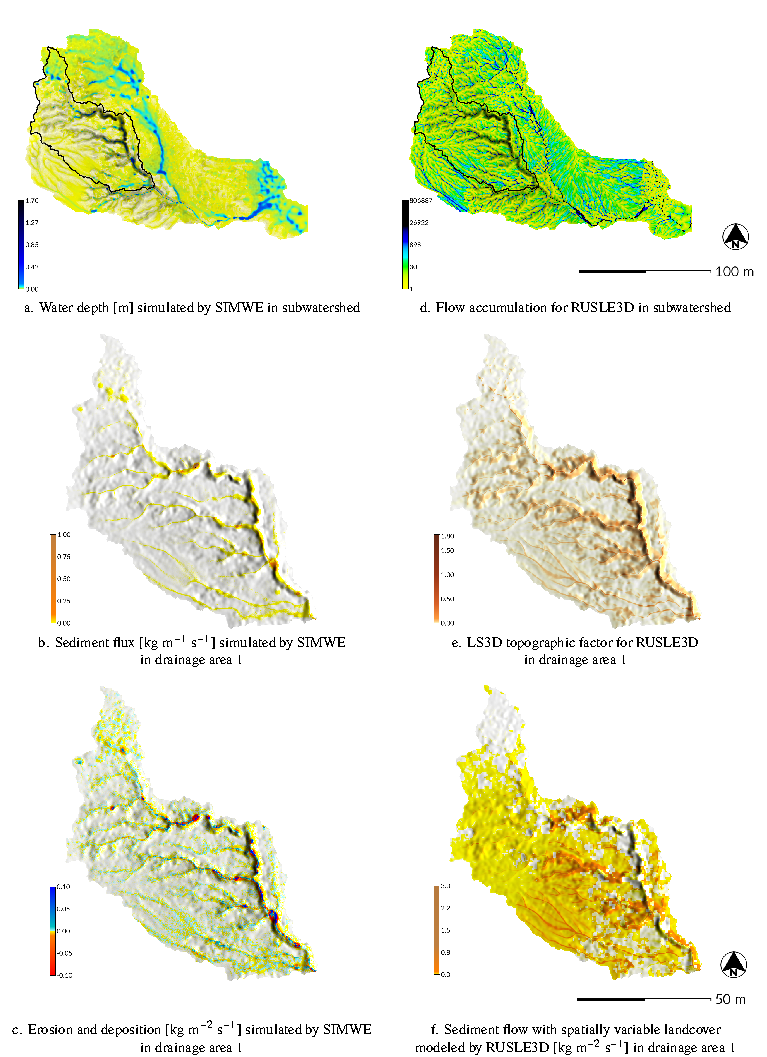
\includegraphics[width=\textwidth,height=0.95\textheight,keepaspectratio]{figures/models.pdf}
\caption{Water and sediment flows 
\DIFaddbeginFL \DIFaddFL{modeled by (a \& c) SIMWE and (b \& d) RUSLE3D with spatially variable landcover 
for a (a \& b) subwatershed and (c \& d) drainage area of Patterson Branch, Fort Bragg, NC.
(a) Water depth }[\DIFaddFL{m}] \DIFaddendFL simulated by SIMWE for a 10~\unit{min} event with 50~\unit{mm~hr}$^{-1}$ \DIFaddbeginFL \DIFaddFL{in the subwatershed.
(b) Flow accumulation for RUSLE3D in the subwatershed.
(c) Erosion }\DIFaddendFL and \DIFaddbeginFL \DIFaddFL{deposition }[\unit{kg~m}\DIFaddFL{$^{-2}$~}\unit{s}\DIFaddFL{$^{-1}$}] \DIFaddFL{simulated by SIMWE in drainage area 1.
(d) Erosion }[\unit{kg~m}\DIFaddFL{$^{-2}$~}\unit{s}\DIFaddFL{$^{-1}$}] \DIFaddFL{modeled }\DIFaddendFL by RUSLE3D \DIFdelbeginFL \DIFdelFL{with a R-factor of 310
}\DIFdelendFL \DIFaddbeginFL \DIFaddFL{in drainage area 1.
}\DIFaddendFL }
\label{fig:models}
\end{figure}

%DIF <  -------------------------- EROSION-DEPOSITION -----------------------------
%DIF >  -------------------------- MATH FOUNDATIONS OF THE MODEL -----------------------------
\DIFaddbegin 

\DIFaddend \subsection{\DIFdelbegin \DIFdel{Simulation of water erosion model}\DIFdelend \DIFaddbegin \DIFadd{Landscape evolution}\DIFaddend }
\DIFaddbegin 

\DIFadd{Landscape evolution in r.sim.terrain 
is driven by the change in the elevation surface 
caused by soil erosion and deposition.
During storm events overland flow erodes soil, 
transports sediment across landscape, and 
under favorable conditions deposits the sediment. 
Gravitational diffusion, 
applied to the changing elevation surface, 
simulates the smoothing effects 
of localized soil transport between events.
}

\subsubsection{\DIFadd{Elevation change}} 
\DIFadd{Assuming negligible uplift, the change in elevation over time 
is described by the continuity of mass equation 
expressed as the divergence of sediment flow  \citep{Tucker2001}:
%DIF >  landscape evolution equation
}\begin{equation}
\DIFadd{\label{eq:evolution} 
}{\DIFadd{\partial z \over \partial t }} \DIFadd{= -\nabla \cdot }{\DIFadd{\bf q_s}} \DIFadd{= d_s ~ \rho_s^{-1} 
}\end{equation}
{\small
\DIFadd{where: }\\
\noindent
\DIFadd{\hspace*{0.5em} $z$ is elevation }[\unit{m}] \\
\DIFadd{\hspace*{0.5em} $t$ is time }[\unit{s}] \\
\DIFadd{\hspace*{0.5em} ${\bf q_s}$ is sediment flow per unit width (vector) }[\unit{kg~m}\DIFadd{$^{-1}$~}\unit{s}\DIFadd{$^{-1}$}]\\
\DIFadd{\hspace*{0.5em} $d_s$ is the net erosion-deposition rate }[\unit{kg~m}\DIFadd{$^{-2}$~}\unit{s}\DIFadd{$^{-1}$}]\\
\DIFadd{\hspace*{0.5em} $\rho_s$ is sediment mass density }[\unit{kg~m}\DIFadd{$^{-3}$}]\DIFadd{.}\\
}
\DIFadd{The net erosion-deposition rate $d_s$ driven by overland flow
in r.sim.terrain is estimated at different levels of complexity based 
on the simulation mode selected by the user.
Gravitational diffusion is then applied to the changed topography 
to simulate the smoothing effects 
of localized soil transport between rainfall events.
The change in elevation due to gravitational diffusion
is a function of the sediment mass density,
the diffusion coefficient, and Laplacian of the elevation
%DIF > -- i.e.~the sum of the second order derivatives of elevation
\citep{Thaxton2004}:
%DIF >  change in elevation (m) = elevation (m) - (change in time (s) / sediment mass density (kg/m^3) * gravitational diffusion coefficient (m^2/s) * divergence (m^-1))
}\begin{equation}
\DIFadd{\label{eq:grav_diffusion} 
}{\DIFadd{\partial z \over \partial t }} \DIFadd{= \rho_s^{-1} ~ \varepsilon_g ~ \nabla^2 z 
}\end{equation}
%DIF > HM this should be \nabla^2 z, \nabla is an operator so there should be a variable upon which it is applied
%DIF > HM see eq 4.41 in Thaxton, also from Willgoose, the second term
\noindent
\DIFadd{where $\varepsilon_g$ is the diffusion coefficient }[\unit{kg~m}\DIFadd{$^{2}$~}\unit{s}\DIFadd{$^{-1}$}]\DIFadd{.
%DIF > HM we can write $\varepsilon_g=c~\varepsilon$ where k[kg] to keep the diffusion coef units the same as in literature
%DIF > If it is the same time step we have
%DIF > \begin{equation}
%DIF > \label{eq:evolution_disc1} 
%DIF > z_{t + \Delta t} = z_t + \Delta z_s + \Delta z_g 
%DIF > \end{equation}
%DIF > if the time step advances we need two equations, something like this: or see Thaxton
%DIF > HM VERIFY whether this is acceptable
}

\noindent
\DIFadd{The discrete implementation follows \cite{Thaxton2004}:
}\begin{equation}
\DIFadd{\label{eq:evolution_disc1} 
z_{t+ \Delta t_1} = z_t + \Delta z_s  
}\end{equation}
\begin{equation}
\DIFadd{\label{eq:evolution_disc2} 
z_{t+\Delta t_1+\Delta t_2} = z_{t+\Delta t_1} + \Delta z_g 
}\end{equation}
{\small
\DIFadd{where: }\\
\noindent
\DIFadd{\hspace*{0.5em} $\Delta z_s$ is elevation change caused by net erosion or deposition
}[\unit{m}] \DIFadd{(Eq.~\ref{eq:evolution})}\\
\DIFadd{\hspace*{0.5em} $\Delta z_g$ is the diffusion driven elevation change
}[\unit{m}] \DIFadd{(Eq.~\ref{eq:grav_diffusion})}\\
\DIFadd{\hspace*{0.5em} $\Delta t_1$ is the time interval during a storm event }[\unit{s}]\\
\DIFadd{\hspace*{0.5em} $\Delta t_2$ is the time interval between events
when gravitational diffusion changes the elevation surface }[\unit{s}]\DIFadd{.}\\
}

\subsubsection{\DIFadd{Erosion-deposition regimes}}

%DIF > In general, the net erosion-deposition $d_s$ is obtained 
%DIF > by solving the sediment transport continuity equation
%DIF > which for the simpler, steady state case relates $d_s$ to the divergence 
%DIF > of sediment flow rate per unit width ${\bf q_s}$ [\unit{kg~m}$^{-1}$~\unit{s}$^{-1}$]:
%DIF > \begin{equation}
%DIF > \label{eq:steady_sed}
%DIF > d_s = \nabla\cdot {\bf q_s} 
%DIF > \end{equation}
\DIFadd{Following experimental observations and qualitative arguments, 
\cite{Foster1977} proposed that the sum of 
the ratio of the net erosion-deposition rate $d_s$ 
to detachment capacity  $D_c$  }[\unit{kg~m}\DIFadd{$^{-2}$~}\unit{s}\DIFadd{$^{-1}$}] 
\DIFadd{and the ratio of the sediment flow rate $q_s = |{\bf q_s}|$ 
to sediment transport capacity $T_c$ }[\DIFadd{$\unit kg~m^{-1}~s^{-1}$}]
\DIFadd{is a conserved quantity (unity):
}\begin{equation}
\DIFadd{\label{eq:foster_law}
}{\DIFadd{d_s \over D_c}} \DIFadd{+ }{\DIFadd{q_s \over T_c}} \DIFadd{= 1
}\end{equation}
\DIFadd{The net erosion and deposition rate $d_s$ can then be expressed 
as being proportional to the difference between
the sediment transport capacity $T_c$ 
and the actual sediment flow rate $q_s$:
}\begin{equation}
\DIFadd{\label{eq:sigma}
d_s = }{\DIFadd{D_c \over T_c}}\DIFadd{~\bigl( T_c - q_s\bigr)
}\end{equation}
\noindent
\DIFadd{This principle is used in several erosion models 
including the Water Erosion Prediction Project (WEPP) \citep{Flanagan2013} 
and SIMWE \citep{Mitas1998}. 
}

\DIFadd{Using this concept it is possible to identify 
two limiting erosion-deposition regimes.
When $T_c >> D_c$ leading to $T_c >> q_s$, 
the erosion regime is detachment capacity limited and
net erosion is equal to the detachment capacity:
}\begin{equation}
\DIFadd{\label{eq:detachment_limited}
 d_s = D_c
}\end{equation}
\DIFadd{For this case the transport capacity of overland flow 
exceeds the detachment capacity 
and thus sediment flow, erosion, and sediment transport
are limited by the detachment capacity. 
Therefore, no deposition occurs.
%DIF > When rainfall intensity is very high ($i_r \geq 60 \unit{mm~hr}^{-1}$)
An example of this case is when a strong storm 
producing intense %DIF >  high 
overland flow over compacted clay soils 
causes high capacity flows to transport light clay particles,
while the detachment of compacted soils is limited.
%DIF > 
When $D_c >> T_c$, sediment flow is at sediment transport capacity $q_s = T_c$, 
leading to a transport capacity limited regime 
with deposition reaching its maximum extent for the given water flow. 
Net erosion-deposition is computed as the divergence of
transport capacity multiplied by a unit vector $\vec{s_0}$ 
in the direction of flow:
}\begin{equation}
\DIFadd{\label{eq:transport_limited}
 d_s = \nabla\cdot (T_c ~ \vec{s_0})
}\end{equation}
%DIF > This would be the case when rainfall intensity is not very high ($i_r < 60 \unit{mm~hr}^{-1} $) and 
\DIFadd{This case may occur, for example, during a moderate storm 
with overland flow over sandy soils 
with high detachment capacity, but low transport capacity.
%DIF > 
For $0 < ({D_c / T_c}) < \infty$ 
the spatial pattern of net erosion-deposition is variable 
and depends on the difference between the sediment transport capacity 
and the actual sediment flow rate at the given location.
}

\DIFadd{The detachment capacity $D_c $  and the sediment-transport capacity $T_c $  
are estimated using shear stress and stream power equations respectively
expressed as power functions of water-flow properties and slope angle.    
%DIF > For a given rainfall rate and surface roughness, these two variables can be derived from a DEM
%DIF > using topographic analysis functions to compute the slope 
%DIF > and flow-routing tools to compute the upslope contributing area 
%DIF > as an input for estimating unit water flow.
The relation between the topographic parameters 
of well known empirical equations for erosion modeling, 
such as USLE and stream power, were presented by \citep{Moore1986} 
and used to develop simple, GIS-based models for limiting erosion-deposition cases 
such as RUSLE3D and USPED \citep{Mitasova2001}.
The SIMWE model estimates $T_c$ and $D_c$ using modified 
equations and parameters developed for the WEPP model 
\citep{Flanagan2013,Mitasova2001}.
}

\DIFadd{The simulation modes in r.sim.terrain include:
} \begin{itemize} 
  \item \DIFadd{the process-based SIMWE model 
  for steady state and unsteady shallow overland flow 
  in variable erosion-deposition regimes
  with $d_s$ computed by solving the shallow water flow 
  and sediment transport continuity equations,
  }\item \DIFadd{the RUSLE3D model for detachment capacity limited cases
  with $d_s$ given by Eq.~(\ref{eq:detachment_limited}),
  }\item \DIFadd{and the USPED model for transport capacity limited regimes
  with $d_s$ given by Eq.~(\ref{eq:transport_limited}).
} \end{itemize} 

\noindent \DIFadd{The following sections explain the computation of $d_s$ for these three modes in more detail.
}

%DIF >  -------------------------- SIMWE -----------------------------
\subsection{\DIFadd{Simulation of Water Erosion (SIMWE)}} \DIFaddend \label{simwe}
%DIF <  simwe intro
SIMWE \DIFdelbegin \DIFdel{-- the Simulation of Water Erosion model -- 
}\DIFdelend is a physics-based simulation of shallow overland water and sediment flow
that uses a path sampling method to solve the continuity \DIFdelbegin \DIFdel{and momentum }\DIFdelend equations 
with a 2D diffusive wave approximation 
\citep{Mitas1998,Mitasova2004}.
SIMWE has been implemented in GRASS GIS as the modules 
r.sim.water
and r.sim.sediment. 
\DIFdelbegin %DIFDELCMD < 

%DIFDELCMD < %%%
\DIFdelend % overview
In SIMWE mode for each \DIFaddbegin \DIFadd{landscape evolution }\DIFaddend time step
r.sim.terrain\DIFdelbegin \DIFdel{determines the soil erosion regime,
simulates water and sediment flows, 
and then evolves the topography. 
%DIF <  erdep
In an variable erosion-deposition regime 
the model 
computes the }\DIFdelend \DIFaddbegin \DIFadd{:
} \begin{itemize} 
\item \DIFadd{computes the first order }\DIFaddend partial derivatives of the \DIFdelbegin \DIFdel{topography,
}\DIFdelend \DIFaddbegin \DIFadd{elevation surface
$\partial z / \partial x$ and $\partial z / \partial y$,
%DIF >  using the GRASS GIS module r.slope.aspect (see the equations in \cite{hofierka2009}),
}\item \DIFaddend simulates shallow water flow \DIFdelbegin \DIFdel{and }\DIFdelend \DIFaddbegin \DIFadd{depth, sediment flow, and the net }\DIFaddend erosion-deposition \DIFdelbegin \DIFdel{,
}\DIFdelend \DIFaddbegin \DIFadd{rate, 
}\item \DIFaddend and then evolves the topography based on the erosion-deposition rate and gravitational diffusion. 
%DIF <  transport limited
\DIFdelbegin \DIFdel{The same process is used in
a transport capacity limited regime,
except that the topography is evolved based on 
the transport limited erosion-deposition rate
and gravitational diffusion.
%DIF <  detachment  limited
In a detachment capacity limited regime
the model instead
computes the }\DIFdelend \DIFaddbegin  \end{itemize} 
%DIF > 
\DIFadd{The first order }\DIFaddend partial derivatives of the \DIFdelbegin \DIFdel{topography,
simulates shallow water flow and sediment flow,
and then evolves the topography based on the sediment flow rate
and gravitational diffusion.
%DIF <  dynamic versus steady state
The model simulates dynamic landscape evolution 
when the }\DIFdelend \DIFaddbegin \DIFadd{elevation surface
are computed using the GRASS GIS module r.slope.aspect 
using the equations in \cite{Hofierka2009}.
r.sim.terrain simulates unsteady-state flow regimes
when the landscape evolution }\DIFaddend time step is less than the travel time 
for a drop of water or a particle of sediment to cross the landscape\DIFaddbegin \DIFadd{,
e.g.~when the time step is less than the time to concentration for the modeled watershed}\DIFaddend .
With longer \DIFaddbegin \DIFadd{landscape evolution }\DIFaddend time steps the model simulates \DIFdelbegin \DIFdel{steady state dynamics}\DIFdelend \DIFaddbegin \DIFadd{a steady state regime}\DIFaddend . 

% ------------------------------------------------------------------------------

\subsubsection{\DIFdelbegin \DIFdel{Erosion regime}\DIFdelend \DIFaddbegin \DIFadd{Shallow water flow}\DIFaddend }

%DIF <  Erosion regime
\DIFdelbegin \DIFdel{This model can switch erosion regimes at each time step
based on the rainfall intensity ($i_r$)
and the balance of the sediment detachment capacity ($D_c$)
and the sediment transport capacity ($T_c$)
represented by the first order reaction term $\sigma$, which depends on soiland landcoverproperties.
The detachment capacity is the maximum potential 
detachment rate by overland flow, 
while
the sediment transport capacity 
is the maximum potential sediment flow rate.
When rainfall intensity is very high ($i_r \geq 60 \unit{mm~hr}^{-1}$)
or $\sigma$ is low ($\sigma \leq 0.01 \unit{m}^{-1}$),
then the regime is detachment capacity limited.%DIF < 
When rainfall intensity is not very high ($i_r < 60 \unit{mm~hr}^{-1} $)and $\sigma$ is high ($\sigma \geq 100 \unit{m}^{-1}$) ,
then the regime is transport capacity limited. 
%DIF < 
When rainfall intensity is not very high 
($i_r<60 \unit{mm~hr}^{-1}$)
and $\sigma$ is neither high nor low 
($ 0.01 \unit{m}^{-1}< \sigma < 100 \unit{m}^{-1}$),
then there is an variable erosion-deposition regime. }%DIFDELCMD < \\
%DIFDELCMD < %%%
%DIF <  erosion regime eq.
%\begin{displaymath}
%\DIFdel{%DIFDELCMD < \label{eq:regime}%%%
%$\sigma = }{\DIFdel{D_c \over T_c}}$
%\end{displaymath}
%DIFAUXCMD
\DIFdelend %DIF >  Shallow water flow
\DIFaddbegin \DIFadd{The SIMWE model simulates shallow overland water flow
controlled by spatially variable topographic, soil, landcover, 
and rainfall parameters by solving the water flow continuity equation 
using a Green's function Monte Carlo path sampling method:
%DIF >  shallow water flow eq.
}\begin{equation}
\DIFadd{\label{eq:water}
%DIF > {\partial h \over \partial t} =
\nabla \cdot \vec{q} = i_e
}\end{equation}
\DIFaddend {\small
\noindent
\DIFdelbegin \DIFdel{where: }\DIFdelend \DIFaddbegin \DIFadd{where: }\DIFaddend \\
\noindent
%DIF > \hspace*{0.5em} $x, y$ is the position [\unit{m}]\\
%DIF > \hspace*{0.5em} $t$ is the time [\unit{s}] \\
%DIF > \hspace*{0.5em} $h$ is the depth of overland flow [\unit{m}]\\
\hspace*{0.5em} \DIFdelbegin \DIFdel{$\sigma$  is a first order reaction term }\DIFdelend \DIFaddbegin \DIFadd{$i_e$ is the rainfall excess rate }\DIFaddend [\DIFdelbegin \DIFdel{$\unit{m}^{-1}$}%DIFDELCMD < ]%%%
\DIFdelend \DIFaddbegin \DIFadd{$\unit{m~s^{-1}}$}]
\DIFadd{(i.e.~rainfall intensity $-$ infiltration $-$ vegetation intercept)}\DIFaddend \\
%DIF > \hspace*{0.5em} $\nabla$ is the divergence operator\\
\hspace*{0.5em} \DIFdelbegin \DIFdel{$D_c$ is the sediment detachment capacity }\DIFdelend \DIFaddbegin \DIFadd{$\vec{q}$ is the water flow per unit width (vector) }\DIFaddend [\DIFdelbegin \DIFdel{$\unit{kg~m}^{-1}s^{-1}$}\DIFdelend \DIFaddbegin \DIFadd{$\unit{m}^2~\unit{s}^{-1}$}\DIFaddend ]\DIFaddbegin \DIFadd{. 
}}

\noindent
\DIFadd{The path sampling method solves the continuity equation 
through the accumulation of the evolving source over the given time period. 
This accumulation process can be interpreted as
an approximation of a dynamic solution with diffusive wave effects
incorporated by adding a diffusion term proportional to
$ \nabla^2 [h^{5/3}]$
in the solution:
}\begin{equation}
\DIFadd{\label{eq:difwater}
-}{\DIFadd{\varepsilon_w\over 2 }}\DIFadd{\nabla^2 ~ h^{5/3}
+\nabla \cdot \vec{q} = i_e
}\end{equation}
{\small
\noindent
 \DIFadd{where: }\DIFaddend \\
 \DIFaddbegin \noindent
 \DIFaddend \hspace*{0.5em} \DIFdelbegin \DIFdel{$T_c$ is the sediment transport capacity }\DIFdelend \DIFaddbegin \DIFadd{$\varepsilon_w$ is a spatially variable diffusion coefficient }\DIFaddend [\DIFdelbegin \DIFdel{$\unit{kg~m}^{-1}s^{-1}$}\DIFdelend \DIFaddbegin \DIFadd{$\unit{m}^{4/3}~\unit{s}^{-1}$}\DIFaddend ]\DIFaddbegin \DIFadd{. }\DIFaddend \\
}
\DIFdelbegin %DIFDELCMD < 

%DIFDELCMD < %%%
%DIF <  ------------------------------------------------------------------------------
%DIFDELCMD < 

%DIFDELCMD < %%%
\subsubsection{\DIFdel{Shallow water flow}}
%DIFAUXCMD
\addtocounter{subsubsection}{-1}%DIFAUXCMD
%DIFDELCMD < 

%DIFDELCMD < %%%
%DIF <  Shallow water flow
\DIFdel{The SIMWE model
simulates shallow overland water flow controlled by spatially variable topographic, soil, landcover, 
and rainfall parameters
by solving the continuity and momentum equations 
for steady state water flow with a path sampling method
(Fig. 
~\ref{fig:models}a ). 
Shallow water flow $q$ can be approximated by
the bivariate form of }\DIFdelend \DIFaddbegin \DIFadd{See \cite{Mitasova2004} for more details 
on this equation and its numerical solution.
The solution assumes that water flow velocity 
is largely controlled by }\DIFaddend the \DIFdelbegin \DIFdel{St.
~Venant equation:
%DIF <  shallow water flow eq.
}
%\begin{displaymath}
%\DIFdel{%DIFDELCMD < \label{eq:water}%%%
%}{\DIFdel{\partial h \over \partial t}} \DIFdel{=
% i_e - \nabla ~ q
%}\end{displaymath}
%DIFAUXCMD
\DIFdelend \DIFaddbegin \DIFadd{slope of the terrain and surface roughness 
and that its change at a given location during the simulated event is negligible. 
The water depth $h$ at time $\tau$ during the simulated rainfall event
%DIF > HM note that we have several time steps in r.sim.terrain 
%DIF > - topo evolution time step, water flow time step and sediment flow time step
 is computed as a function of particle (walkers) density at each grid cell. 
The initial number of particles per grid cell 
is proportional to the rainfall excess rate $i_e$ (source).
Particles are then routed across the landscape 
by finding a new position for each walker at time $\tau + \Delta \tau$:
}\begin{equation}
\DIFadd{\vec{r}_m^{new}=\vec{r}_m + \Delta \tau \vec{v} + \vec{g}
}\end{equation}

\DIFaddend {\small
\noindent
where: \\
\noindent
\hspace*{0.5em} \DIFdelbegin \DIFdel{$x, y$ is the }\DIFdelend \DIFaddbegin \DIFadd{$\vec{r} = (x, y)$ is the $m^{th}$ walker }\DIFaddend position [\unit{m}]\\
\hspace*{0.5em} \DIFdelbegin \DIFdel{$t$ is the time }\DIFdelend \DIFaddbegin \DIFadd{$\Delta \tau$ is the particle routing time step }\DIFaddend [\unit{s}]\\
\hspace*{0.5em} \DIFdelbegin \DIFdel{$h$ is the depth of overland flow }\DIFdelend \DIFaddbegin \DIFadd{$\vec{g}$ is a random vector with gaussian components with variance $\Delta \tau$ }\DIFaddend [\unit{m}]\\
\hspace*{0.5em} \DIFdelbegin \DIFdel{$i_e$ is the rainfall excess }\DIFdelend \DIFaddbegin \DIFadd{$\vec{v} $ is the water flow velocity vector }\DIFaddend [\DIFdelbegin %DIFDELCMD < \unit{m~s^{-1}}%%%
\DIFdelend \DIFaddbegin \DIFadd{$\unit{m~s^{-1}}$}\DIFaddend ]
\DIFdelbegin %DIFDELCMD < \\
%DIFDELCMD < %%%
\DIFdel{\hspace*{0.5em} (i.e.~rainfall intensity $-$ infiltration $-$ vegetation intercept)}%DIFDELCMD < \\
%DIFDELCMD < %%%
\DIFdel{\hspace*{0.5em} $\nabla$ is the divergence of the flow vector field}%DIFDELCMD < \\
%DIFDELCMD < %%%
\DIFdel{\hspace*{0.5em} $q$ is the water flow per unit width }\DIFdelend \DIFaddbegin \DIFadd{whose magnitude is computed with the Manning's equation $v=n^{-1}~h^{2/3}~s^{1/2}$ 
where $n$ is the Manning's coefficient }\DIFaddend [\DIFdelbegin \DIFdel{$\unit{m}^2~\unit{s}^{-1}$}\DIFdelend \DIFaddbegin \DIFadd{$\unit{s~m^{-1/3}}$}\DIFaddend ] \DIFaddbegin \DIFadd{and $s$ is slope}\DIFaddend .\\ 
}
\DIFdelbegin %DIFDELCMD < 

%DIFDELCMD < %%%
\DIFdelend %DIF > 
\noindent
\DIFdelbegin \DIFdel{Diffusive wave effects can be approximated
so that water can flow through depressions 
by integrating a diffusion term 
$ \propto \nabla^2 [h^{5/3}]$
into the solution of the continuity and momentum equations 
for steady state water flow .
This equation
is solved }\DIFdelend \DIFaddbegin \DIFadd{The mathematical background of the method,
including the incorporation of approximate momentum 
through an increased diffusion rate in the prevailing direction of flow,
is presented by \cite{Mitas1998} and \cite{Mitasova2004}.
}

%DIF > ADD COMPUTATION OF WALKER DENSITY HERE 

%DIF >  ------------------------------------------------------------------------------
\subsubsection{\DIFadd{Sediment flow and net erosion-deposition}}

%DIF >  Sediment flow
\DIFadd{The SIMWE model simulates the sediment flow over complex topography 
with spatially variable overland flow, soil, and landcover properties 
by solving  the sediment flow continuity equation
}\DIFaddend using a Green's function Monte Carlo path sampling method.
%DIF <   diffuse wave eq.
%\DIFdelbegin \begin{displaymath}
%\DIFdel{%DIFDELCMD < \label{eq:difwater}%%%
%-}
%{\DIFdel{\varepsilon\over 2 }}\DIFdel{\nabla^2 }[\DIFdel{h^{5/3}}]
%\DIFdel{+\nabla ~ }[ \DIFdel{h~v}] \DIFdel{= i_e
%}\end{displaymath}
%DIFAUXCMD
%DIFDELCMD < {\small
%DIFDELCMD < \noindent
%DIFDELCMD <  %%%
\DIFdel{where: }%DIFDELCMD < \\
%DIFDELCMD <  \noindent
%DIFDELCMD <  %%%
\DIFdel{\hspace*{0.5em} $\varepsilon$ is a spatially variable diffusion coefficient. }%DIFDELCMD < \\
%DIFDELCMD < }
%DIFDELCMD < 

%DIFDELCMD < %%%
%DIF <  ------------------------------------------------------------------------------
%DIFDELCMD < 

%DIFDELCMD < %%%
\subsubsection{\DIFdel{Sediment flow}}
%DIFAUXCMD
\addtocounter{subsubsection}{-1}%DIFAUXCMD
%DIFDELCMD < 

%DIFDELCMD < %%%
%DIF <  Sediment flow
\DIFdel{In SIMWE the }\DIFdelend \DIFaddbegin \DIFadd{Steady state sediment flow $\vec{q_s}$ is approximated by
the bivariate continuity equation, which relates 
the change in }\DIFaddend sediment flow rate \DIFdelbegin \DIFdel{$q_s$ is estimated
as }\DIFdelend \DIFaddbegin \DIFadd{to effective sources and sinks:
%DIF > 
}\begin{equation}
\DIFadd{\label{eq:steady_sed}
\nabla\cdot \vec{q_s} = }{\DIFadd{\rm sources - sinks}}\DIFadd{= d_s
}\end{equation}
%DIF > 
\noindent
\DIFadd{The sediment-flow rate $\vec{q_s}$ is }\DIFaddend a function of water flow and sediment concentration
\citep{Mitas1998}\DIFdelbegin \DIFdel{(Fig.~\ref{fig:models}b): %DIF < sediment flow equation
}
%\begin{displaymath}\DIFdel{%DIFDELCMD < \label{eq:sedflow} %%%
%q_s=\rho_s ~ q
%}\end{displaymath}
%%DIFAUXCMD
%\DIFdelend 
\DIFaddbegin \DIFadd{: %DIF > (Fig.~\ref{fig:models}b)
%DIF > 
}\begin{equation}
\DIFadd{\label{eq:sedflow}
\vec{q_s} = \rho_s~c~\vec{q} = \rho_s~c~h~\vec{v} = \varrho~\vec{v}
}\end{equation}
\DIFaddend {\small
\noindent
where: \\
\hspace*{0.5em} \DIFdelbegin \DIFdel{$q_s$ is the sediment flow rate per unit width }\DIFdelend \DIFaddbegin \DIFadd{$\rho_s$ is sediment mass density in the water column }\DIFaddend [\unit{kg~m}\DIFdelbegin \DIFdel{$^{-1}$~}%DIFDELCMD < \unit{s}%%%
\DIFdel{$^{-1}$}\DIFdelend \DIFaddbegin \DIFadd{$^{-3}$}\DIFaddend ]\\
\hspace*{0.5em} \DIFdelbegin \DIFdel{$\rho_s$ is sediment mass density }\DIFdelend \DIFaddbegin \DIFadd{$c$ is sediment concentration }\DIFaddend [\DIFdelbegin %DIFDELCMD < \unit{kg~m}%%%
\DIFdel{$^{-3}$}\DIFdelend \DIFaddbegin \DIFadd{$\unit{particle~m^{-3}}$}\DIFaddend ]\DIFdelbegin \DIFdel{.}\DIFdelend \\
\DIFaddbegin \DIFadd{\hspace*{0.5em} $\varrho = \rho_s~c~h$ is the mass of sediment transported by water per unit area }[\DIFadd{$\unit{kg~m^{-2}}$}]\DIFadd{. 
}\DIFaddend }

%DIF <  ------------------------------------------------------------------------------
\DIFdelbegin %DIFDELCMD < 

%DIFDELCMD < %%%
\subsubsection{\DIFdel{Erosion-deposition}}
%DIFAUXCMD
\addtocounter{subsubsection}{-1}%DIFAUXCMD
%DIFDELCMD < 

%DIFDELCMD < %%%
%DIF <  Erosion-deposition
\DIFdel{In SIMWE 
the net erosion-deposition rate is estimated
using the bivariate form of sediment continuity equation
to model sediment storage and flow based on effective sources and sinks
(Fig.~\ref{fig:models}c). 
Net erosion-deposition $d_s$
-- the difference between sources and sinks --
is approximated by
the steady state sediment flow equationwith diffusion :
%DIF <  erosion-deposition equation
}
%\begin{displaymath}\DIFdel{%DIFDELCMD < \label{eq:sediment} %%%
%d_s = 
%}{\DIFdel{\partial }[\DIFdel{\rho_s ~ h}] \DIFdel{\over \partial t}} \DIFdel{+
%\nabla~q_s
%}\end{displaymath}
%DIFAUXCMD
\DIFdelend \DIFaddbegin \DIFadd{The sediment flow equation (\ref{eq:steady_sed}),
like the water flow equation, 
has been rewritten to include a small diffusion term that is
proportional to the mass of water-carried sediment per unit area 
$\nabla^2 \varrho$ \citep{Mitas1998}:
}\begin{equation}
\DIFadd{\label{eq:difsedim}
-}{\DIFadd{\varepsilon_s \over 2}}\DIFadd{\nabla^2 \varrho
+ \nabla\cdot }[\DIFadd{\varrho \vec{v}}]
 \DIFadd{+ \varrho~}{\DIFadd{D_c \over T_c}}\DIFadd{~|}{\DIFadd{\bf v}}\DIFadd{|
= D_c
%DIF > \sigma(\vec{r}) T(\vec{r})=Dc/T * T=Dc
}\end{equation}
\DIFaddend {\small
\noindent
where:\\
\DIFdelbegin \DIFdel{\hspace*{0.5em} $d_s$ is net erosion-deposition }\DIFdelend \DIFaddbegin \noindent
\DIFadd{\hspace*{0.5em} $\varepsilon_s$ is the diffusion constant }\DIFaddend [\DIFdelbegin %DIFDELCMD < \unit{kg~m}%%%
\DIFdel{$^{-2}$~}%DIFDELCMD < \unit{s}%%%
\DIFdel{$^{-1}$}\DIFdelend \DIFaddbegin \DIFadd{$\unit{m^2~s^{-1}}$}\DIFaddend ].\\
}

%DIF <  ------------------------------------------------------------------------------
\DIFdelbegin %DIFDELCMD < 

%DIFDELCMD < %%%
\subsubsection{\DIFdel{Landscape evolution}}
%DIFAUXCMD
\addtocounter{subsubsection}{-1}%DIFAUXCMD
%DIFDELCMD < 

%DIFDELCMD < %%%
%DIF <  Landscape evolution
\DIFdel{The simulated change in elevation $\Delta z$
due to water erosion and deposition
is a function of the change in time, 
the net erosion-deposition rate}\DIFdelend \DIFaddbegin \DIFadd{On the left hand side of equation \ref{eq:difsedim}, 
the first term describes local diffusion, 
the second term is drift driven by the water flow}\DIFaddend ,
and the \DIFdelbegin \DIFdel{sediment mass density 
\citep{Mitasova2013}:
%DIF <  landscape evolution equation
}
%\begin{displaymath}
%\DIFdel{%DIFDELCMD < \label{eq:evolution} %%%
%}{\DIFdel{\Delta z = \Delta t ~ d_s ~ \rho_s^{-1} }}
%\end{displaymath}
%DIFAUXCMD
%DIFDELCMD < 

%DIFDELCMD < %%%
%DIF <  detachment limited landscape evolution
\DIFdelend \DIFaddbegin \DIFadd{third term represents a velocity dependent `potential'
acting on the mass of transported sediment. 
%DIF > The equation is solved for $\varrho$ which is represented by particle density.
The initial number of particles per grid cell 
is proportional to the soil detachment capacity $D_c$ (source).
The particles are then routed across the landscape
by finding a new position for each the walker at time $\tau + \Delta \tau$:
}\begin{equation}
\DIFadd{\vec{r}_m^{new}=\vec{r}_m + \Delta \tau \vec{v} + \vec{g}
}\end{equation}
\DIFadd{while the updated weight is:
}\begin{equation}
\DIFadd{w_m^{new}=w_m \exp[- \Delta \tau(u(\vec{r}_m^{new})+u(\vec{r}_m))/2]
}\end{equation}
{\small
\DIFaddend \noindent
\DIFdelbegin \DIFdel{In a detachment limited erosion regime
the simulated change in elevation $\Delta z$
is a function of
the change in time , the }\DIFdelend \DIFaddbegin \DIFadd{where:}\\
\noindent
\DIFadd{\hspace*{0.5em} $u = {D_c / T_c}~|\vec{v}|$.}\\
}
%DIF > 
\noindent
%DIF > The sediment flow rate is computed as weighted particle densities 
%DIF > multiplied by the unit vector in the direction of flow
\DIFadd{The }\DIFaddend sediment flow rate \DIFdelbegin \DIFdel{, and the mass of water carried sediment per unit area
\citep{Mitasova2013}:
%DIF <  change in elevation (m) = change in time (s) * sediment flux (kg/ms) / mass of sediment per unit area (kg/m^2)
}
%\begin{displaymath}
%\DIFdel{\label{eq:flux_evolution} 
%}
%{\DIFdel{\Delta z = \Delta t ~ q_s~ \varrho_s^{-1} }} 
%\end{displaymath}
%DIFAUXCMD
\DIFdelend \DIFaddbegin \DIFadd{is computed 
as the product of weighted particle densities 
and the unit vector in the direction of flow
$\vec{q_s} = \varrho~\vec{s_0}$.  %DIF > VERIFY 
Then net erosion-deposition $d_s$ 
is computed as the divergence of sediment flow using equation (\ref{eq:steady_sed}).
}

\DIFadd{SIMWE estimates the detachment capacity $D_c $ and 
the sediment-transport capacity $T_c $ 
as functions of shear stress and stream power respectively. 
Specifically,  the detachment capacity is:
}\begin{equation}
\DIFadd{\label{eq:detach_cap}
D_c =K_d  \bigl(\gamma - \gamma_0 \bigr)^b  
}\end{equation}
\DIFaddend {\small
\noindent
where: \\
\noindent
\hspace*{0.5em} \DIFdelbegin \DIFdel{$\varrho_s$ }\DIFdelend \DIFaddbegin \DIFadd{$K_d$ is the effective erodibility 
(detachment-capacity coefficient) }[\DIFadd{$\unit{s~m^{-1}}$}] \DIFadd{for $b=1$}\\ %DIF > VERIFY
\DIFadd{\hspace*{0.5em} $\gamma=\rho_w~g~h~\sin \beta$ is shear stress }[\DIFadd{$\unit{Pa=kg~m^{-2}}$}] \\
\DIFadd{\hspace*{0.5em} $\rho_w$ }\DIFaddend is the mass \DIFdelbegin \DIFdel{of sediment per unit area }\DIFdelend \DIFaddbegin \DIFadd{density of water }\DIFaddend [\DIFdelbegin %DIFDELCMD < \unit{kg ~ m}%%%
\DIFdel{$^{-2}$}\DIFdelend \DIFaddbegin \DIFadd{$\unit{kg~m^{-3}}$}\DIFaddend ] \DIFdelbegin \DIFdel{.}\DIFdelend \\
\DIFaddbegin \DIFadd{\hspace*{0.5em} $g$ is gravitational acceleration }[\DIFadd{$\unit{m~s^{-2}}$}]\\
\DIFadd{\hspace*{0.5em} $\gamma_0$ is critical shear stress }[\DIFadd{Pa}] \\
\DIFadd{\hspace*{0.5em} $b$ is an empirical exponent.
}\DIFaddend }

%DIF <  ------------------------------------------------------------------------------
\DIFdelbegin %DIFDELCMD < 

%DIFDELCMD < %%%
%DIF <  gravitational diffusion
\DIFdelend \noindent
\DIFdelbegin \DIFdel{Gravitational diffusion is then applied to the evolved topography
to simulate the settling of sediment particles. 
The simulated change in elevation $\Delta z$ %DIF < $\Delta z(x,y,t)$
due to gravitational diffusion 
is }\DIFdelend \DIFaddbegin \DIFadd{Shear stress $\gamma $ is computed
as }\DIFaddend a function of \DIFdelbegin \DIFdel{the change in time, the sediment mass density, 
the gravitational diffusion coefficient, and topographic divergence 
-- i.e.~the sum of the second order derivatives of elevation
\citep{Thaxton2004}:
%DIF <  change in elevation (m) = elevation (m) - (change in time (s) / sediment mass density (kg/m^3) * gravitational diffusion coefficient (m^2/s) * divergence (m^-1))
}
%\begin{displaymath}
%\DIFdel{\label{eq:grav_diffusion} 
%}
%{\DIFdel{\Delta z = \Delta t ~ \rho_s^{-1} ~ \varepsilon_g ~ \nabla}}
%\end{displaymath}
%DIFAUXCMD
\DIFdelend \DIFaddbegin \DIFadd{water depth $h$ estimated by r.sim.water
and the surface slope angle $\beta$ }[\DIFadd{$\unit{\degree}$}]\DIFadd{.
%DIF > 
Sediment-transport capacity is computed as a function 
of unit stream power $\omega$ \citep{Moore1986}:
}\smallskip
\begin{equation}
\DIFadd{\label{eq:tc_streampower}
T_c =K_s \omega = K_s~\gamma~|}{\DIFadd{\bf v}}\DIFadd{| =
K_s~n^{-1}~g_w~h^m~(\sin \beta)^p
}\end{equation}
\DIFaddend {\small
\noindent
where: \\
\noindent
\hspace*{0.5em} \DIFdelbegin \DIFdel{$\varepsilon_g$ is the gravitational diffusion }\DIFdelend \DIFaddbegin \DIFadd{$K_s$ is the effective sediment-transport capacity }\DIFaddend coefficient [\DIFdelbegin %DIFDELCMD < \unit{m}%%%
\DIFdel{$^{2}$~}%DIFDELCMD < \unit{s}%%%
\DIFdel{$^{-1}$}\DIFdelend \DIFaddbegin \DIFadd{s}\DIFaddend ] \\
\hspace*{0.5em} \DIFdelbegin \DIFdel{$\nabla$ is the topographic divergence }%DIFDELCMD < [\unit{m}%%%
\DIFdel{$^{-1}$}%DIFDELCMD < ]%%%
\DIFdel{.
}%DIFDELCMD < \\
%DIFDELCMD < %%%
\DIFdelend \DIFaddbegin \DIFadd{$m$ and $p$ are empirical exponents.
}\DIFaddend }

%DIF > CHECK implementation may have omega just power of gamma without velocity
\DIFaddbegin 

%DIF >  Erosion regime
\DIFadd{This model can simulate erosion regimes 
from prevailing detachment limited conditions when $T_c >> D_c$ 
to prevailing transport capacity limited conditions when $D_c >> T_c$
and the erosion-deposition patterns between these conditions.
At each landscape evolution time step, the regime can change based on 
the ratio between the sediment detachment capacity $D_c$
and the sediment transport capacity $T_c$ and the actual sediment flow rate.
If the landscape evolution time step is shorter than the time to concentration 
(i.e.~the time for water to reach steady state)
then net erosion-deposition is derived from unsteady flow.
}

\DIFaddend % -------------------------------- RUSLE --------------------------------
\subsection{Revised \DIFdelbegin \DIFdel{universal soil loss equation 3D model}\DIFdelend \DIFaddbegin \DIFadd{Universal Soil Loss Equation for Complex Terrain (RUSLE3D)}\DIFaddend }
\label{rusle_model}
\DIFdelbegin \DIFdel{The Revised Universal Soil Loss Equation for Complex Terrain (}\DIFdelend RUSLE3D
\DIFdelbegin \DIFdel{) 
}\DIFdelend is an empirical \DIFdelbegin \DIFdel{equation }\DIFdelend \DIFaddbegin \DIFadd{model }\DIFaddend for computing erosion 
in a detachment capacity limited soil erosion regime
for watersheds with complex topography \citep{Mitasova1996}. 
It is based on 
the Universal Soil Loss Equation (USLE),
an empirical equation for estimating the average
sheet and rill soil erosion from rainfall and runoff
on agricultural fields and rangelands with simple topography 
\citep{Wischmeier1978}. 
It models erosion dominated regimes without deposition
in which sediment transport capacity is 
uniformly greater than detachment capacity.
\DIFdelbegin \DIFdel{As an empirical equation the predicted soil loss 
is spatially and temporally averaged. 
}\DIFdelend In USLE soil loss per unit area is determined by 
an erosivity factor $R$,
a soil erodibility factor $K$, 
a slope length factor $L$,
a slope steepness factor $S$,
a cover management factor $C$,
and a prevention measures factor $P$.
These factors are empirical constants derived 
from an extensive collection of measurements 
on 22.13 \unit{m} standard plots with an average slope of 9$\%$.  
RUSLE3D was designed to account for more complex, 3D topography 
with converging and diverging flows. 
In RUSLE3D the topographic potential for erosion at any given point 
is represented by a 3D topographic factor $LS_{3D}$,
which is a function of the upslope contributing area 
and the angle of the slope. 

In this spatially and temporally distributed model 
RUSLE3D is modified by the use of a 
event-based \DIFdelbegin \DIFdel{r-factor derived from the }\DIFdelend \DIFaddbegin \DIFadd{R-factor derived from }\DIFaddend rainfall intensity at each time step.
For each time step this model computes the parameters for RUSLE3D -- 
an event-based erosivity factor,
the slope of the topography, the flow accumulation, and
the 3D topographic factor -- 
and then solves the RUSLE3D equation for \DIFdelbegin \DIFdel{sediment flow. 
The sediment flow is }\DIFdelend \DIFaddbegin \DIFadd{the rate of soil loss 
(i.e.~the net soil erosion rate). 
The soil erosion rate is then }\DIFaddend used to simulate landscape evolution 
in a detachment capacity limited soil erosion regime.

%DIF <  RESOURCES
%DIF <  https://ncsu-geoforall-lab.github.io/erosion-modeling-tutorial/erdep_theory.html
%DIF <  http://www4.ncsu.edu/~hmitaso/gmslab/reports/CerlErosionTutorial/denix/denixstart.html
\DIFdelbegin %DIFDELCMD < 

%DIFDELCMD < %%%
\DIFdelend % ------------------------------------------------------------------------------

\subsubsection{\DIFdelbegin \DIFdel{Event-based erosivity }\DIFdelend \DIFaddbegin \DIFadd{Erosivity }\DIFaddend factor}

The erosivity factor $R$ in USLE and RUSLE 
is the combination of the total energy 
and peak intensity of a rainfall event,
representing the interaction 
between the detachment of sediment particles
and the transport capacity of the flow. 
It can be calculated as the product of the 
the kinetic energy of the rainfall event $E$
and its maximum 30 \unit{min} intensity $I_{30}$
\DIFdelbegin \DIFdel{\citep{Brown1987,Renard1997}}\DIFdelend \DIFaddbegin \DIFadd{\citep{Brown1987,Renard1997,Panagos2015,Panagos2017}}\DIFaddend .
In this model, however, the erosivity factor
is derived at each time step as a function of
kinetic energy, rainfall \DIFdelbegin \DIFdel{volume}\DIFdelend \DIFaddbegin \DIFadd{depth}\DIFaddend , rainfall intensity, and time.
First rain energy is derived from rainfall intensity \DIFdelbegin \DIFdel{\citep{Brown1987}:
%DIF < 
}
%\begin{displaymath}
%\DIFdel{\label{eq:rain_energy}
%}{\DIFdel{e_r = 0.29 ~ (1.-0.72 ~ exp(-0.05 ~ i_r))}}
%\end{displaymath}
%DIFAUXCMD
\DIFdelend \DIFaddbegin \DIFadd{\citep{Brown1987,Yin2017}:
%DIF > VERIFY UNITS FOR ALL EQS BELOW:
}

\begin{equation}
\DIFadd{\label{eq:rain_energy}
}{\DIFadd{e_r \over e_0}} \DIFadd{= 1.- b ~ exp\bigl(}{\DIFadd{i_r \over i_0}} \DIFadd{\bigr)
}\end{equation}
\DIFaddend %
{\small
\noindent
where: \\
\noindent
\hspace*{0.5em} $e_r$is unit rain energy [\unit{MJ~ha}$^{-1}$~\unit{mm}${^-1}$]\\
\hspace*{0.5em} $i_r$ is rainfall intensity [\unit{mm~h}$^{-1}$]\DIFdelbegin \DIFdel{.}\DIFdelend \\
\DIFaddbegin \DIFadd{\hspace*{0.5em} $b$ is empirical coeficient}\\
\DIFadd{\hspace*{0.5em} $i_0$ is reference rainfall intensity }[\unit{mm~h}\DIFadd{$^{-1}$}]\\
\DIFadd{\hspace*{0.5em} $e_0$ is reference energy }[\unit{MJ~ha}\DIFadd{$^{-1}$~}\unit{mm}\DIFadd{${^-1}$}]\DIFadd{. 
}\DIFaddend }

\noindent
\DIFaddbegin \DIFadd{The parameters for this equation were derived from observed data
published for different regions by \cite{Panagos2017}.
%DIF >  erosivity per time step
}\noindent
\DIFaddend Then the event-based erosivity index $R_e$ 
is calculated as the product of 
unit rain energy, rainfall \DIFdelbegin \DIFdel{volume}\DIFdelend \DIFaddbegin \DIFadd{depth}\DIFaddend , rainfall intensity, and time: 
%\DIFdelbegin \begin{displaymath}
%\DIFdel{\label{eq:erosivity_index}
%}{\DIFdel{R_e = e_r ~ v_r ~ i_r ~ t_r}}
%\end{displaymath}
%%DIFAUXCMD
%\DIFdelend 
\DIFaddbegin \begin{equation}
\DIFadd{\label{eq:erosivity_index}
}{\DIFadd{R_e = e_r ~ v_r ~ i_r ~ \Delta t}}
\end{equation}
\DIFaddend %
{\small
\noindent
where: \\
\hspace*{0.5em} $R_e$ is the event-based erosivity index [\unit{MJ~mm~ha}$^{-1}$~\unit{hr}$^{-1}$]\\
\hspace*{0.5em} $v_r$ is the rainfall \DIFdelbegin \DIFdel{volume }\DIFdelend \DIFaddbegin \DIFadd{depth }\DIFaddend [\unit{mm}] derived from \DIFdelbegin \DIFdel{${v_r = i_r~t_r}$}\DIFdelend \DIFaddbegin \DIFadd{${v_r = i_r~\Delta t}$}\DIFaddend \\
\hspace*{0.5em} \DIFdelbegin \DIFdel{$t_r$ is the time interval }\DIFdelend \DIFaddbegin \DIFadd{$\Delta t$ is the change in time }\DIFaddend [\unit{s}].
}


%DIF >  --------------------------- EI_30 ---------------------------------------
\DIFaddbegin 

%DIF > % single storm erosivity
%DIF > \noindent The erosivity of a single rainfall event $EI_{30}$
%DIF > divided into $m$ total periods
%DIF > can be calculated as
%DIF > \citep{Panagos2015,Panagos2017}:
%DIF > %
%DIF > \begin{equation}
%DIF > \label{eq:erosivity_index}
%DIF > EI_{30} = \Bigg(\sum_{r=1}^{m}~ e_r ~ v_r \Bigg) ~ I_{30}
%DIF > \end{equation}
%DIF > %
%DIF > {\small
%DIF > \noindent
%DIF > where: \\
%DIF > \hspace*{0.5em} $EI_{30}$ is the rainfall erosivity index of a single event [\unit{MJ~mm~ha}$^{-1}$~\unit{hr}$^{-1}$]\\
%DIF > \hspace*{0.5em} $e_r$ is the unit rainfall energy [\unit{MJ~ha}$^{-1}$~\unit{mm}$^{-1}$]\\
%DIF > \hspace*{0.5em} $v_r$ is the rainfall volume [\unit{mm}] during time period $r$\\
%DIF > \hspace*{0.5em} $I_{30}$ is the maximum rainfall intensity during a 30-min period of the rainfall event [\unit{mm}~\unit{hr}$^{-1}$].
%DIF > }
%DIF > %
%DIF > \noindent In this model, however, the erosivity factor
%DIF > is derived at each time step $r$ as a function of
%DIF > kinetic energy ($e_r$), rainfall volume ($v_r$), rainfall intensity ($i_r$). 
%DIF > First rain energy is derived from rainfall intensity \citep{Brown1987}: 

%DIF > \begin{equation}
%DIF > \label{eq:rain_energy}
%DIF > {e_r = 0.29 ~ (1.-0.72 ~ exp(-0.05 ~ i_r))}
%DIF > \end{equation}
%DIF > %
%DIF > {\small
%DIF > \noindent
%DIF > where: \\
%DIF > \noindent
%DIF > \hspace*{0.5em} $e_r$is unit rain energy [\unit{MJ~ha}$^{-1}$~\unit{mm}${^-1}$]\\
%DIF > \hspace*{0.5em} $i_r$ is rainfall intensity [\unit{mm~h}$^{-1}$].\\
%DIF > }

%DIF > % erosivity per time step
%DIF > \noindent
%DIF > Then the erosivity per time step %$EI_r$ 
%DIF > is calculated as the product of 
%DIF > unit rain energy, rainfall volume, rainfall intensity, and time:  
%DIF > %
%DIF > \begin{equation}
%DIF > \label{eq:erosivity_index}
%DIF > EI_{r} = e_r ~ v_r ~ i_{r}
%DIF > \end{equation}
%DIF > %
%DIF > {\small
%DIF > \noindent
%DIF > where: \\
%DIF > \hspace*{0.5em} $EI_r$ is the rainfall erosivity during time $r$ [\unit{MJ~mm~ha}$^{-1}$~\unit{hr}$^{-1}$].
%DIF > %\hspace*{0.5em} $e_r$ is the unit rainfall energy [\unit{MJ~ha}$^{-1}$~\unit{mm}$^{-1}$]\\
%DIF > %\hspace*{0.5em} $v_r$ is the rainfall volume [\unit{mm}] during time period $r$\\
%DIF > %\hspace*{0.5em} $i_r$ is the rainfall intensity during time period $r$ [\unit{mm}~\unit{hr}$^{-1}$].
%DIF > }

\DIFaddend % ------------------------------------------------------------------------------

\subsubsection{Flow accumulation}
%
The upslope contributing area per unit width \DIFaddbegin \DIFadd{$a$
}\DIFaddend is determined by flow accumulation 
\DIFdelbegin \DIFdel{times }\DIFdelend \DIFaddbegin \DIFadd{(the number of grid cells draining into a given grid cell)
multiplied by }\DIFaddend grid cell width (Fig.~\ref{fig:models}d). 
Flow accumulation is calculated using 
a multiple flow direction algorithm \citep{Metz2009} 
based on $A^{T}$ least cost path searches \citep{Ehlschlaeger1989}. 
The multiple flow direction algorithm 
implemented in GRASS GIS as the module r.watershed
is computationally efficient\DIFaddbegin \DIFadd{, does not require sink filling, 
}\DIFaddend and can navigate nested depressions and other obstacles. 

% ------------------------------------------------------------------------------

\subsubsection{3D topographic factor}
%DIF < 
The 3D topographic factor \DIFdelbegin \DIFdel{$LS_{3D}(x,y)$
}\DIFdelend \DIFaddbegin \DIFadd{$LS_{3D}$
}\DIFaddend is calculated as a function of the \DIFdelbegin \DIFdel{flow accumulation,
representing the }\DIFdelend upslope contributing area
\DIFdelbegin \DIFdel{,
}\DIFdelend and the slope (Fig.~\ref{fig:models}e). 
%DIF < 
\DIFdelbegin \DIFdel{The empirical coefficients $m$ and $n$
for the upslope contributing area 
and the slope
can range from 0.2 to 0.6
and 1.0 to 1.3 respectively
with low values representing dominant sheet flow
and high values representing dominant rill flow.
%DIF < 
}
%\begin{displaymath}
%\DIFdel{\label{eq:ls_factor}
%}{\DIFdel{LS_{3D} = (m+1.0) ~ (a(x,y) ~ a_0^{-1})^{m} ~ (sin(\beta) ~ \beta_0^{-1})^{n}}}
%\end{displaymath}
%DIFAUXCMD
\DIFdelend 
%\DIFaddbegin \begin{equation}
%\DIFadd{\label{eq:ls_factor}
%LS_{3D} = (m+1) ~ \left(}{\DIFadd{a \over a_0}}\DIFadd{\right)^m ~ \left(}{\DIFadd{\sin \beta \over \beta_0}}\DIFadd{\right)^n
%}\end{equation}
%\DIFaddend %
{\small
\noindent
where: \\
\noindent
\hspace*{0.5em} $LS_{3D}$ is the dimensionless topographic \DIFdelbegin \DIFdel{(length-slope) }\DIFdelend factor\\
\hspace*{0.5em} $a$ is upslope contributing area per unit width [\unit{m}]\\
\hspace*{0.5em} $a_0$ is the length of the standard USLE plot [22.1 \unit{m}]\\
\hspace*{0.5em} $\beta$ is the angle of the slope [$\degree$]\\
\hspace*{0.5em} $m$ is an empirical coefficient\\
\hspace*{0.5em} $n$ is an empirical coefficient\\
\hspace*{0.5em} $\beta_0$ is the slope of the standard USLE plot [0.09$\degree$]\DIFaddbegin \DIFadd{.}\DIFaddend \\
}
\DIFaddbegin \DIFadd{The empirical coefficients $m$ and $n$
for the upslope contributing area and the slope
can range from 0.2 to 0.6 and 1.0 to 1.3 respectively
with low values representing dominant sheet flow
and high values representing dominant rill flow.
}\DIFaddend %RESOURCES: http://www4.ncsu.edu/~hmitaso/gmslab/papers/erijgis.html

% ------------------------------------------------------------------------------

\subsubsection{\DIFdelbegin \DIFdel{Sediment flow}\DIFdelend \DIFaddbegin \DIFadd{Detachment limited erosion rate}\DIFaddend }

\DIFdelbegin \DIFdel{Sediment flow }\DIFdelend \DIFaddbegin \DIFadd{The erosion rate }\DIFaddend is a function of the event-based erosivity factor, 
\DIFdelbegin \DIFdel{the }\DIFdelend soil erodibility factor, \DIFdelbegin \DIFdel{the }\DIFdelend 3D topographic factor,
\DIFdelbegin \DIFdel{cover }\DIFdelend \DIFaddbegin \DIFadd{landcover }\DIFaddend factor, and \DIFdelbegin \DIFdel{the }\DIFdelend prevention measures factor 
(Fig.~\ref{fig:models}\DIFdelbegin \DIFdel{f}\DIFdelend \DIFaddbegin \DIFadd{d}\DIFaddend ):
%
\begin{equation}
\label{eq:rusle}
{E = R_e ~ K ~ LS_{3D} ~ C ~ P}
\end{equation}
%
{\small
\noindent
where: \\
\noindent
\hspace*{0.5em} $E$ is \DIFdelbegin \DIFdel{sediment flow }\DIFdelend \DIFaddbegin \DIFadd{soil erosion rate (soil loss) }\DIFaddend [\unit{kg~m}$^{-2}$~\unit{min}$^{-1}$]\\
\hspace*{0.5em} $R_e$ is the event-based erosivity factor [\unit{MJ~mm~ha}$^{-1}$~\unit{hr}$^{-1}$]\\
\hspace*{0.5em} $K$ is the soil erodibility factor [\unit{ton~ha~hr~ha}$^{-1}$~\unit{MJ}$^{-1}$~\unit{mm}$^{-1}$]\\
\hspace*{0.5em} $LS_{3D}$ is the dimensionless topographic (length-slope) factor\\
\hspace*{0.5em} $C$ is the dimensionless \DIFdelbegin \DIFdel{land cover }\DIFdelend \DIFaddbegin \DIFadd{landcover }\DIFaddend factor\\
\hspace*{0.5em} $P$ is the dimensionless prevention measures factor.\\
}

% Landscape evolution
\noindent
\DIFdelbegin \DIFdel{For }\DIFdelend \DIFaddbegin \DIFadd{The detachment limited erosion represented by }\DIFaddend RUSLE3D \DIFaddbegin \DIFadd{leads to }\DIFaddend the simulated change in elevation\DIFdelbegin \DIFdel{$\Delta z$
is derived from 
equation \ref{eq:flux_evolution}
for landscape evolution in an detachment limited soil erosion regime
and then equation \ref{eq:grav_diffusion}for the settling of sediment particles due to }\DIFdelend \DIFaddbegin \DIFadd{: 
}\begin{equation}
\DIFadd{\label{eq:dz_rusle}
}{\DIFadd{\Delta z_s = D_c \rho_s^{-1} = E ~ \rho_s^{-1}}}
\end{equation}
\DIFadd{which is combined with Eq. (\ref{eq:grav_diffusion})
for }\DIFaddend gravitational diffusion.

% -------------------------------- USPED --------------------------------

\subsection{Unit \DIFdelbegin \DIFdel{streampower erosion deposition model}\DIFdelend \DIFaddbegin \DIFadd{Streampower Erosion Deposition (USPED)}\DIFaddend } \label{usped_model}
\DIFdelbegin \DIFdel{The Unit Stream Power Erosion Deposition (USPED ) model 
}\DIFdelend \DIFaddbegin \DIFadd{USPED }\DIFaddend estimates net erosion-deposition as the divergence of sediment flow
in transport capacity limited soil erosion \DIFdelbegin \DIFdel{regimes.
At transport capacity 
shallow flows of water are carrying as much sediment possible 
-- more sediment is being detached than can be transported}\DIFdelend \DIFaddbegin \DIFadd{regime.
The amount of soil detached is 
close to the amount of sediment that water flow can carry}\DIFaddend .
As a transport capacity limited model
USPED predicts erosion where transport capacity increases
and deposition where transport capacity decreases. 
The influence of topography on \DIFdelbegin \DIFdel{erosion and deposition in USPED 
}\DIFdelend \DIFaddbegin \DIFadd{sediment flow  
}\DIFaddend is represented by a topographic sediment transport factor,
while the influence of soil and landcover are represented by 
factors adopted from USLE and RUSLE
\citep{Mitasova1996}.
%
\DIFdelbegin \DIFdel{Net erosion-deposition }\DIFdelend \DIFaddbegin \DIFadd{Sediment flow }\DIFaddend is estimated by computing
the event-based erosivity factor ($R_e$) 
using Eq.~\ref{eq:erosivity_index},
the slope and aspect of the topography,
the flow accumulation with a multiple flow direction algorithm,
the topographic sediment transport factor,
\DIFdelbegin \DIFdel{the }\DIFdelend \DIFaddbegin \DIFadd{and }\DIFaddend sediment flow at transport capacity\DIFdelbegin \DIFdel{,
and }\DIFdelend \DIFaddbegin \DIFadd{.
Net erosion-deposition is then computed as }\DIFaddend the divergence of \DIFdelbegin \DIFdel{the }\DIFdelend sediment flow. 

% Topographic sediment transport factor
\DIFdelbegin \DIFdel{The }\DIFdelend \DIFaddbegin \DIFadd{Using the unit stream power concept presented by \cite{Moore1986},
the }\DIFaddend 3D topographic factor (Eq.~\ref{eq:ls_factor}) 
for RUSLE3D is \DIFdelbegin \DIFdel{adapted }\DIFdelend \DIFaddbegin \DIFadd{modified }\DIFaddend to represent 
the topographic sediment transport factor (\DIFdelbegin \DIFdel{$LST$}\DIFdelend \DIFaddbegin \DIFadd{$LS_T$}\DIFaddend ) --
the topographic component 
of overland flow at sediment transport capacity:
%
\DIFdelbegin 
%\begin{displaymath}
%\DIFdel{\label{eq:lst_factor}
%}{\DIFdel{LST = a^{m} ~ (\sin \beta)^{n}}}
%\end{displaymath}
%DIFAUXCMD
\DIFdelend \DIFaddbegin \begin{equation}
\DIFadd{\label{eq:lst_factor}
}{\DIFadd{LS_T = a^{m} ~ (\sin \beta)^{n}}}
\end{equation}
\DIFaddend %
{\small
\noindent
where: \\
\noindent
\hspace*{0.5em} \DIFdelbegin \DIFdel{$LST$ }\DIFdelend \DIFaddbegin \DIFadd{$LS_T$ }\DIFaddend is the topographic sediment transport factor\\
\hspace*{0.5em} $a$ is the upslope contributing area per unit width [\DIFdelbegin \DIFdel{m}\DIFdelend \DIFaddbegin \unit{m}\DIFaddend ]\\
\hspace*{0.5em} $\beta$ is the angle of the slope [$\degree$]\\
\hspace*{0.5em} $m$ is an empirical coefficient\\
\hspace*{0.5em} $n$ is an empirical coefficient.\\
}

% Sediment flow at transport capacity
\noindent
\DIFdelbegin \DIFdel{The sediment }\DIFdelend \DIFaddbegin \DIFadd{Sediment }\DIFaddend flow at transport capacity is a function of 
the event-based rainfall factor, \DIFdelbegin \DIFdel{the }\DIFdelend soil erodibility factor, 
\DIFdelbegin \DIFdel{the }\DIFdelend topographic component of overland flow,
\DIFdelbegin \DIFdel{the }\DIFdelend landcover factor, and \DIFdelbegin \DIFdel{the }\DIFdelend prevention measures factor:
%
\DIFdelbegin 
%\begin{displaymath}
%\DIFdel{%DIFDELCMD < \label{eq:usped}%%%
%}{\DIFdel{T = R_e ~ K ~ C ~ P ~ LST}}
%\end{displaymath}
%DIFAUXCMD
\DIFdelend \DIFaddbegin \begin{equation}
\DIFadd{\label{eq:usped}
}{\DIFadd{T = R_e ~ K ~ C ~ P ~ LS_T}}
\end{equation}
\DIFaddend {\small
\noindent
where: \\
\noindent
\hspace*{0.5em} $T$ is sediment flow at transport capacity [\unit{kg~m}$^{-1}$~\unit{s}$^{-1}$]\\ 
\hspace*{0.5em} $R_e$ is the event-based rainfall factor [\unit{MJ~mm~ha}$^{-1}$~\unit{hr}$^{-1}$]\\
\hspace*{0.5em} $K$ is the soil erodibility factor [\unit{ton~ha~hr~ha}$^{-1}$~\unit{MJ}$^{-1}$~\unit{mm}$^{-1}$]\\ 
\hspace*{0.5em} $C$ is the dimensionless land cover factor\\
\hspace*{0.5em} $P$ is the dimensionless prevention measures factor.\\
}

%Erosion-deposition at transport capacity
\noindent
Net erosion-deposition \DIFdelbegin \DIFdel{at transport capacity }\DIFdelend is estimated as the divergence of sediment flow\DIFaddbegin \DIFadd{, 
assuming that sediment flow is equal to sediment transport capacity}\DIFaddend : 
%D = ∇ · (T s0) = ∂(T cos α)/∂x + ∂(T sin α)/∂y
\begin{equation}\label{eq:usped_erdep} 
d_s = 
{\partial (T ~ \cos \alpha) \over \partial x} +
{\partial (T ~ \sin \alpha) \over \partial y}
\end{equation}
{\small
\noindent
where: \\
\hspace*{0.5em} $d_s$ is net erosion-deposition [\unit{kg~m}$^{-2}$~\unit{s}$^{-1}$]\\
\hspace*{0.5em} $\alpha$ is the aspect of the topography \DIFaddbegin \DIFadd{(i.e.~the direction of flow) }\DIFaddend [$\degree$].\\
}

%Landscape evolution
\noindent
With USPED the simulated change in elevation \DIFdelbegin \DIFdel{$\Delta z$
}\DIFdelend \DIFaddbegin \DIFadd{$\Delta z_s=d_s$
}\DIFaddend is derived from equation \ref{eq:evolution} for landscape evolution
and then equation \ref{eq:grav_diffusion}
for \DIFdelbegin \DIFdel{the settling of sediment particles due to }\DIFdelend gravitational diffusion.

% -------------------------------- CASE STUDIES --------------------------------

\section{Case study} 

Military activity is a high-impact land use 
that can cause significant physical alteration to the landscape. 
Erosion is a major concern for military installations, 
particularly at training bases, 
where the land surface is disturbed by 
off-road vehicles, foot traffic, and munitions. 
Off-road vehicles and foot traffic by soldiers 
cause the loss of vegetative cover, 
the disruption of soil structure, soil compaction, 
and increased runoff due to 
reduced soil capacity for water infiltration 
\citep{Webb1983, McDonald2004}.
Gullies -- ephemeral channels with steep headwalls 
that incise into unconsolidated soil to depths of meters -- 
are a manifestation of erosion common to 
military training installations like Ft. Bragg in North Carolina 
and the \DIFdelbegin \DIFdel{Piñon }\DIFdelend \DIFaddbegin \DIFadd{Pi\~{n}on }\DIFaddend Canyon Maneuver Site in Colorado. 
While the local development of gullies can restrict 
the maneuverability of troops and vehicles during training exercises, 
pervasive gullying across a landscape 
can degrade an entire training area 
\citep{Huang2014}.

To test the effectiveness of the different models 
in r.sim.terrain
we compared the simulated evolution
of a highly eroded subwatershed of 
Patterson Branch \DIFdelbegin \DIFdel{Creek }\DIFdelend on Fort Bragg, North Carolina
against a timeseries of airborne lidar surveys.
The models -- SIMWE, RUSLE3D, and USPED --
were tested in steady state and dynamic modes
for \DIFdelbegin \DIFdel{constant rainfall, design storms , and recorded rainfall.
}\DIFdelend \DIFaddbegin \DIFadd{design storms with constant rainfall.
%DIF > for constant rainfall, design storms, and recorded rainfall.
}\DIFaddend 

\subsection{Patterson Branch\DIFdelbegin \DIFdel{Creek}\DIFdelend }

\begin{figure}
\DIFdelbeginFL %DIFDELCMD < \centering
%DIFDELCMD < \begin{overpic}[width=0.75\textwidth]{../images/sample_data_3d/naip_2014.png}
%DIFDELCMD < \put(0,0){\includegraphics[height=65mm,center]{../images/sample_data_3d/map_elements.png}}  
%DIFDELCMD < \end{overpic} \\
%DIFDELCMD < %%%
\DIFdelendFL \DIFaddbeginFL \center
\includegraphics[width=\textwidth,height=0.95\textheight,keepaspectratio]{figures/watershed.pdf}
\DIFaddendFL \caption{Subwatershed with 2014 orthoimagery
\DIFaddbeginFL \DIFaddFL{(a) }\DIFaddendFL draped over \DIFaddbeginFL \DIFaddFL{the }\DIFaddendFL 2016 digital elevation model
\DIFaddbeginFL \DIFaddFL{and (b) drainage areas with 2014 orthoimagery}\DIFaddendFL , Patterson Branch\DIFdelbeginFL \DIFdelFL{Creek}\DIFdelendFL , Fort Bragg, NC, USA}
\DIFdelbeginFL %DIFDELCMD < %DIFDELCMD < \label{fig:3d}%%%
%DIFDELCMD < %%%
\DIFdelendFL \DIFaddbeginFL \label{fig:watershed}
\DIFaddendFL \end{figure}

With 650~\unit{km}$^{2}$ of land
Fort Bragg is the largest military installation in the US
and has extensive areas of bare, erodible soils
on impact areas, firing ranges, landing zones, and dropzones. 
It is located in the Sandhills region of North Carolina 
with a Longleaf Pine and Wiregrass Ecosystem \citep{Sorrie2006}.
%
The study landscape 
-- a subwatershed of Patterson Branch \DIFdelbegin \DIFdel{Creek 
}\DIFdelend \DIFaddbegin \DIFadd{(Figure~\ref{fig:watershed}a) 
}\DIFaddend in the Coleman Impact Area --
is pitted with impact craters from artillery and mortar shells
and has an active, approximately 2~\unit{m} deep gully. 
%
It is a Pine-Scrub Oak Sandhill community
composed primarily of Longleaf Pine (\DIFdelbegin \DIFdel{Pinus palustris}\DIFdelend \DIFaddbegin \DIFadd{\emph{Pinus palustris}}\DIFaddend )
and Wiregrass (\DIFdelbegin \DIFdel{Aristida stricta}\DIFdelend \DIFaddbegin \DIFadd{\emph{Aristida stricta}}\DIFaddend )
on Blaney and Gilead loamy sands 
\citep{Sorrie2004}. 
%
Throughout the Coleman Impact Area
frequent fires ignited by live munitions
drive the ecological disturbance regime
of this fire adapted ecosystem.
%
In 2016 the  450~\unit{m}$^{2}$ study site was
43.24\% bare ground with predominately loamy sands,
39.54\% covered by the Wiregrass community, and
17.22\% forested with the Longleaf Pine community 
(Figure~\ref{fig:study_area}\DIFdelbegin \DIFdel{c}\DIFdelend \DIFaddbegin \DIFadd{a}\DIFaddend ). 
%
We hypothesize that the elimination of forest cover
in the impact zone
triggered extensive channelized overland flow,
gully formation, and sediment transport into the creek. 

% --------- DATA ---------
Timeseries of digital elevations models 
and landcover maps for the study landscape
were generated from lidar pointclouds and orthophotography\DIFdelbegin \DIFdel{(Figure~\ref{fig:study_area}a-c).
}\DIFdelend \DIFaddbegin \DIFadd{.
%DIF > (Figure~\ref{fig:study_area}a-c). 
}\DIFaddend The digital elevations models for 2004, 2012, and 2016
were interpolated at \DIFdelbegin \DIFdel{0.3}\DIFdelend \DIFaddbegin \DIFadd{1}\DIFaddend ~\unit{m} resolution
using the regularized spline with tension function \citep{Mitasova1993,Mitasova2005}
from airborne lidar surveys 
collected by the NC Floodplain Mapping program and Fort Bragg. 
%
Unsupervised image classification 
was used to identify clusters of spectral reflectance
in a timeseries of 1~\unit{m} resolution orthoimagery 
collected by the National Agriculture Imagery Program.
The landcover maps were derived \DIFdelbegin \DIFdel{by fusing }\DIFdelend \DIFaddbegin \DIFadd{from }\DIFaddend the
classified lidar point clouds \DIFdelbegin \DIFdel{with }\DIFdelend \DIFaddbegin \DIFadd{and }\DIFaddend the classified orthoimagery.
Spatially variable soil erosion factors 
-- \DIFaddbegin \DIFadd{the }\DIFaddend k-factor, c-factor, \DIFdelbegin \DIFdel{mannings}\DIFdelend \DIFaddbegin \DIFadd{Manning's coefficient}\DIFaddend , and runoff \DIFdelbegin \DIFdel{rates }\DIFdelend \DIFaddbegin \DIFadd{rate }\DIFaddend --
were \DIFaddbegin \DIFadd{then }\DIFaddend derived from the landcover and soil maps.
The dataset for this study is hosted at 
\url{https://github.com/baharmon/landscape\_evolution_dataset}
under the ODC Open Database License (ODbL).
The data is derived from publicly available data from
the US Army, USGS, USDA, Wake County GIS, NC Floodplain
Mapping Program, and the NC State Climate Office.
\DIFaddbegin \DIFadd{There are detailed instructions for preparing the input data in the 
}\href{https://github.com/baharmon/landscape_evolution/blob/master/tutorial.md}{tutorial}
\DIFadd{and a complete record of the commands used to process the sample data in the
}\href{https://github.com/baharmon/landscape_evolution_dataset/blob/master/nc_spm_evolution/DATA.md}{data log}\DIFadd{.
}\DIFaddend 

% --------- MORPHOLGY ---------
We used the geomorphons method 
of automated landform classification
based on the openness of terrain \citep{Jasiewicz2013}
and the difference between the digital elevation models 
to analyze the changing morphology of the study area
(Figure~\ref{fig:study_area}\DIFdelbegin \DIFdel{d-f}\DIFdelend \DIFaddbegin \DIFadd{c-d}\DIFaddend ). 
%
The 2~\unit{m} deep gully -- 
its channels classified as valleys and 
its scour pits as depressions by geomorphons -- 
has multiple mature branches
and ends with a depositional fan.
%
The gully has also developed 
depositional ridges beside the channels.
Deep scour pits have developed 
where branches join the main channel 
and where the main channel has sharp bends.
%
A new branch has begun to form 
in a knickzone classified as a mix of valleys and hollows
on a grassy swale on the northeast side of the gully.
Between 2012 and 2016 a depositional ridge
has developed at the foot of this nascent branch
where it would meet the main channel. 
%
The difference in elevation between 2012 and 2016
(Figure~\ref{fig:study_area}\DIFdelbegin \DIFdel{d}\DIFdelend \DIFaddbegin \DIFadd{c}\DIFaddend )
shows a deepening of the main channel 
by approximately 0.2~\unit{m} 
and the scours pits
by approximately 1~\unit{m},
while depositional ridges have formed and grown up to
approximately 1~\unit{m} or more.

% study area figure
\begin{figure}
\center
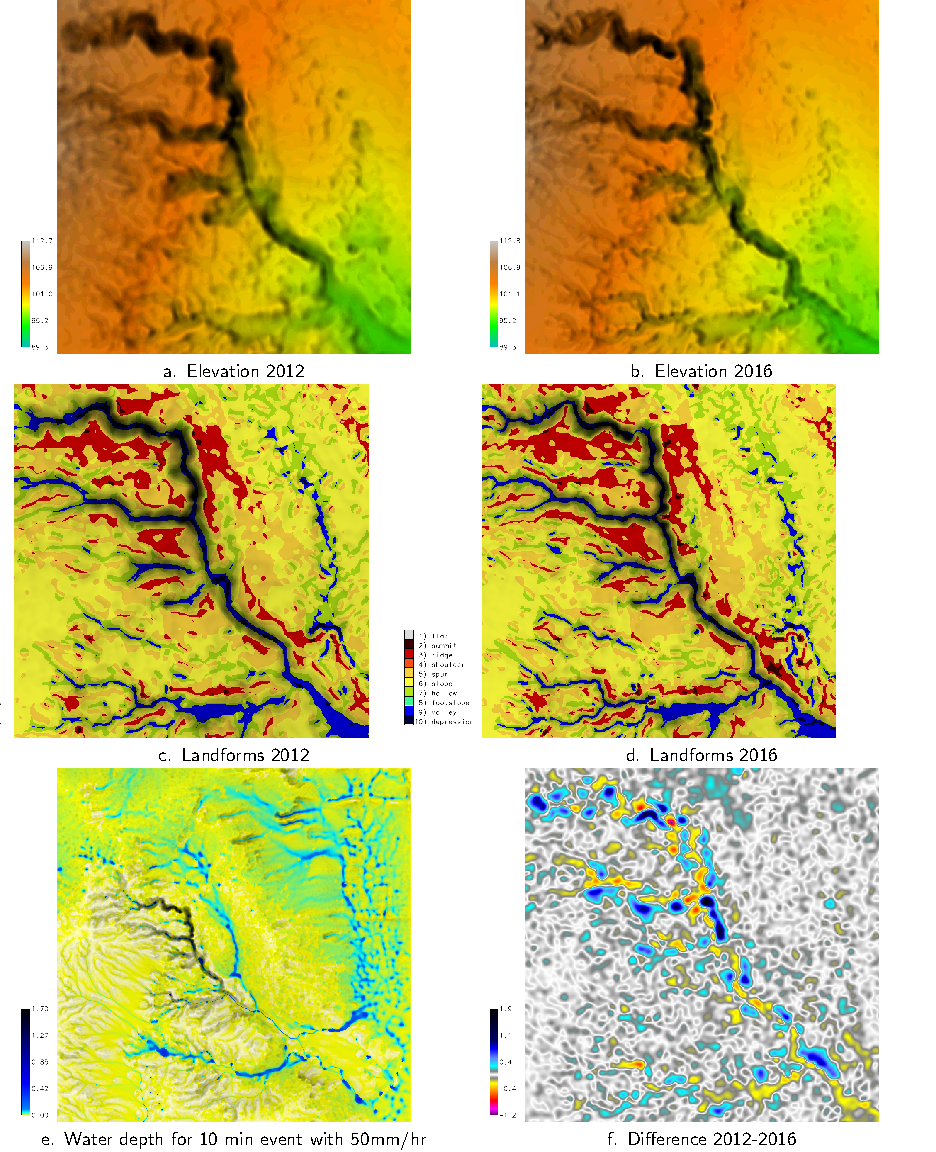
\includegraphics[width=\textwidth,height=0.95\textheight,keepaspectratio]{figures/study_area.pdf}
\caption{\DIFaddbeginFL \DIFaddFL{Morphological Change, Drainage Area 1, Study }\DIFaddendFL Subwatershed, Patterson Branch\DIFdelbeginFL \DIFdelFL{Creek}\DIFdelendFL , Fort Bragg, NC, USA\DIFaddbeginFL \DIFaddFL{.
(a) Landcover in 2014, 
(b) landforms in 2012,
(c) elevation difference between 2012-2016 }[\DIFaddFL{m}]\DIFaddFL{, and
(d) landforms in 2016.
}\DIFaddendFL }
\label{fig:study_area}
\end{figure}

% --------- SIMULATIONS ---------
\subsection{Simulations}
%
We ran a sequence of r.sim.terrain simulations 
\DIFaddbegin \DIFadd{with design storms
}\DIFaddend for the Patterson Branch \DIFdelbegin \DIFdel{Creek }\DIFdelend subwatershed study area
to \DIFdelbegin \DIFdel{test dynamic and steady state flow regimes
in the SIMWE, }\DIFdelend \DIFaddbegin \DIFadd{demonstrate the capabilities 
of the }\DIFaddend RUSLE3D, \DIFdelbegin \DIFdel{and USPED}\DIFdelend \DIFaddbegin \DIFadd{USPED, and SIMWE }\DIFaddend models
(Table~\ref{table:simulations}).
%
\DIFdelbegin \DIFdel{RUSLE3D was used to simulate }\DIFdelend \DIFaddbegin \DIFadd{To analyze the results of the simulations,
we compared 
net differences in elevation
morphological features,
and linear regressions of elevation change.
}

%DIF >  design storms
\DIFadd{While r.sim.terrain can use rainfall records,
we used design storms to demonstrate and test 
the basic capabilities of the model. 
Our design storms are based off the peak rainfall values
in records from the State Climate Office of North Carolina.
%DIF >  parameters
We used RUSLE3D to simulate landscape evolution
in a dynamic, detachment capacity limited soil erosion regime
for a }\DIFaddend 120~\unit{min} \DIFdelbegin \DIFdel{events
with rainfall intensities }\DIFdelend \DIFaddbegin \DIFadd{design storm
with 3~}\unit{min} \DIFadd{intervals 
and a constant rainfall intensity }\DIFaddend of 50~\unit{mm~hr}$^{-1}$
\DIFdelbegin \DIFdel{for detachment capacity limited soil erosion regimes
for both dynamic and steady state flow regimes
using RUSLE3D
}\DIFdelend (Figure~\ref{fig:simulations}\DIFdelbegin \DIFdel{a-c}\DIFdelend \DIFaddbegin \DIFadd{a-b}\DIFaddend ).
%
\DIFdelbegin \DIFdel{USPED was used to simulate 120~}%DIFDELCMD < \unit{min} %%%
\DIFdel{events
with rainfall intensities of }%DIFDELCMD < \unit{50~mm~hr}%%%
\DIFdel{$^{-1}$
for }\DIFdelend \DIFaddbegin \DIFadd{We used USPED to simulate landscape evolution
in a dynamic, }\DIFaddend transport capacity limited soil erosion \DIFdelbegin \DIFdel{regimes
for both dynamic and steady state flow regimes
}\DIFdelend \DIFaddbegin \DIFadd{regime
for a 120~}\unit{min} \DIFadd{design storm
with 3~}\unit{min} \DIFadd{intervals 
and a constant rainfall intensity of 50~}\unit{mm~hr}\DIFadd{$^{-1}$
}\DIFaddend (Figure~\ref{fig:simulations}\DIFdelbegin \DIFdel{d-f}\DIFdelend \DIFaddbegin \DIFadd{c-d}\DIFaddend ).
%
\DIFdelbegin \DIFdel{SIMWE was used to simulate }\DIFdelend \DIFaddbegin \DIFadd{We used SIMWE to simulate landscape evolution
in a steady state, variable erosion-deposition soil erosion regime
for a }\DIFaddend 120~\unit{min} \DIFdelbegin \DIFdel{events 
with rainfall intensities }\DIFdelend \DIFaddbegin \DIFadd{design storm
with a constant rainfall intensity }\DIFaddend of 50~\unit{mm~hr}$^{-1}$
\DIFdelbegin \DIFdel{for erosion-deposition 
and detachment limited soil erosion regimes 
in steady state flow regimes
}\DIFdelend (Figure~\ref{fig:simwe_simulations}\DIFaddbegin \DIFadd{a-b}\DIFaddend ). 
%
In all of the simulations 
a sink filling algorithm
-- an optional parameter in r.sim.terrain -- 
was used to reduce the effects of positive feedback loops
that cause the over-development of scour pits. 

% scripts
The simulations were automated and run in parallel
using Python scripts that are available in the 
\href{https://github.com/baharmon/landscape_evolution}{software repository}.
% reproducibility
The simulations can be reproduced using these scripts
and the study area dataset 
by following the instructions 
in the Open Science Framework repository 
at \url{https://osf.io/tf6yb/}.
% benchmarks
The simulations were run 
in GRASS GIS 7.4 
on a desktop computer 
with 64-bit Ubuntu 16.04.4 LTS,
8 x 4.20 GHz Intel Core i7 7700K CPUs,
and 32 GB RAM. 
% multithreading
Simulations using SIMWE 
are far more computationally intensive
than RULSE3D or USPED, 
but support multi-threading 
when compiled with OpenMP. 
% runtime
Dynamic simulations of RUSLE3D and USPED \DIFdelbegin \DIFdel{each took
}\DIFdelend \DIFaddbegin \DIFadd{took
2~}\unit{min}\DIFadd{~36~}\unit{s} \DIFadd{and 
}\DIFaddend 3~\unit{min}~14~\unit{s} \DIFaddbegin \DIFadd{respectively
}\DIFaddend to run on a single thread, 
while \DIFdelbegin \DIFdel{steady state simulations for SIMWE each took 
84}\DIFdelend \DIFaddbegin \DIFadd{the steady state simulation for SIMWE took 
44}\DIFaddend ~\unit{min}~\DIFdelbegin \DIFdel{13}\DIFdelend \DIFaddbegin \DIFadd{51}\DIFaddend ~\unit{s} running on 6 threads
(Table~\ref{table:simulations}).

%DIF <  --------- RESULTS ---------
\subsection{Results}

%DIF <  dynamic model results
%DIF >  --------- RESULT TABLES ---------
\DIFaddbegin 

%DIF >  table of simulations
\begin{table*}
\small
\caption{\DIFaddFL{Landscape evolution simulations}}
%\begin{tabu} \DIFaddFL{to \textwidth }{\DIFaddFL{XXXXXllllX}}
%\toprule
%\DIFaddFL{Flow regime }& \DIFaddFL{Model }& \DIFaddFL{Intensity }& \DIFaddFL{Duration }& \DIFaddFL{Interval }& \DIFaddFL{m }& \DIFaddFL{n }& \DIFaddFL{$\rho_s$ }& \DIFaddFL{Threads }& \DIFaddFL{Runtime}\\
%\midrule
%\DIFaddFL{Dynamic }& \DIFaddFL{RUSLE3D }& \DIFaddFL{50~}\unit{mm~hr}\DIFaddFL{$^{-1}$ }& \DIFaddFL{120~}\unit{min} & \DIFaddFL{3~}\unit{min} &  \DIFaddFL{0.4 }& \DIFaddFL{1.3 }& & & \DIFaddFL{2~}\unit{min}\DIFaddFL{~36~}\unit{s}\\
%\DIFaddFL{Dynamic }& \DIFaddFL{USPED }& \DIFaddFL{50~}\unit{mm~hr}\DIFaddFL{$^{-1}$ }& \DIFaddFL{120~}\unit{min} & \DIFaddFL{3~}\unit{min} &  \DIFaddFL{1.5 }& \DIFaddFL{1.2 }& \DIFaddFL{1.6 }& & \DIFaddFL{3~}\unit{min}\DIFaddFL{~14~}\unit{s}\\
%\DIFaddFL{Steady state }& \DIFaddFL{SIMWE }& \DIFaddFL{50~}\unit{mm~hr}\DIFaddFL{$^{-1}$ }& \DIFaddFL{120~}\unit{min} & \DIFaddFL{120~}\unit{min} & & & \DIFaddFL{1.6 }& \DIFaddFL{6 }& \DIFaddFL{44~}\unit{min}\DIFaddFL{~51~}\unit{s}\\
%\bottomrule
%\\
%\end{tabu}
\label{table:simulations} 
\end{table*}

%DIF >  linear regression table
\begin{table*}
\small
\caption{\DIFaddFL{Linear regression of elevation maps for drainage area}}
%\begin{tabu} \DIFaddFL{to \textwidth }{\DIFaddFL{lXXl}}
%\toprule
%\DIFaddFL{Elevation A }& \DIFaddFL{Elevation B }&  \DIFaddFL{Correlation coeff. (R) }& \DIFaddFL{Difference in R from 2012-2016 baseline }\\
%\midrule
%\DIFaddFL{2012 }& \DIFaddFL{2016 }& \DIFaddFL{0.999490 }& \DIFaddFL{0}\\
%\DIFaddFL{2012 }& \DIFaddFL{simulated with RUSLE3D }& \DIFaddFL{0.999848 }& \DIFaddFL{-0.000483}\\
%\DIFaddFL{2012 }& \DIFaddFL{simulated with USPED }& \DIFaddFL{0.999973 }& \DIFaddFL{-0.000253}\\
%\DIFaddFL{2012 }& \DIFaddFL{simulated with SIMWE }& \DIFaddFL{0.998312 }& \DIFaddFL{0.001178}\\
%\bottomrule
%\\
%\end{tabu}
\label{table:linear_regression} 
\end{table*}


%DIF >  --------------------------------------------

%DIF > Given the presence the mature gully 
%DIF > with ridges along its banks,
%DIF > this landscape had previously been dominated by 
%DIF > a detachment limited soil erosion regime, but 
%DIF > during our study period it was dominated by
%DIF > a transport capacity limited or 
%DIF > variable erosion-deposition soil erosion regime. 

\DIFaddend The dynamic RUSLE3D simulation
deepened the main channel of the gully,
while the dynamic USPED simulation
eroded the banks of the gully
and deposited in channels
causing the gully grow wider and shallower
(Figure~\ref{fig:simulations}). 
%DIF < 
%DIF >  rusle
As a detachment capacity limited model
RUSLE3D's results were
dominated by erosion and 
thus negative elevation change.
%DIF < 
RUSLE3D carved a deep incision 
in the main gully channel
where water \DIFdelbegin \DIFdel{and sediment flow }\DIFdelend accumulated
(Figure~\ref{fig:simulations}\DIFdelbegin \DIFdel{c). 
%DIF < 
}\DIFdelend \DIFaddbegin \DIFadd{b). 
%DIF >  usped
}\DIFaddend As a transport capacity limited model
USPED generated a distributed pattern
with both erosion and deposition and thus
negative and positive elevation change.
%DIF < 
While USPED's pattern of elevation change
was grainy and fragmented, 
it captured the process of channel 
filling and widening expected with 
a transport capacity limited soil erosion regime
(Figure~\ref{fig:simulations}\DIFdelbegin \DIFdel{f). 
}%DIFDELCMD < 

%DIFDELCMD < %%%
%DIF <  steady state model results
\DIFdelend \DIFaddbegin \DIFadd{d). 
%DIF >  simwe
}\DIFaddend The steady state SIMWE \DIFdelbegin \DIFdel{simulations 
predicted more realistic patterns 
of landscape evolution
(Figure~\ref{fig:simwe_simulations}). 
%DIF < 
For transport limited and
}\DIFdelend \DIFaddbegin \DIFadd{simulation
for a }\DIFaddend variable erosion-deposition \DIFdelbegin \DIFdel{regimes
SIMWE simulated
channel widening}\DIFdelend \DIFaddbegin \DIFadd{regime
predicted the morphological processes and features
expected of its regime including
gradual aggradation,
channel widening,
}\DIFaddend and the formation of depositional ridges
along the thalweg of the channel
(Figure~\ref{fig:simwe_simulations}\DIFdelbegin \DIFdel{c).
%DIF < 
For a detachment limited soil erosion regime
SIMWE simulated major erosion
driving the continued development 
of the gully network
including the spread of rills and
the evolution of the nascent branch
into a full fledged channel
(Figure~\ref{fig:simwe_simulations}f).
%DIF < 
The detachment limited simulation
also formed extensive ridges
beside the gully channels 
(Figure~\ref{fig:simwe_simulations}f), 
continuing the development of channel-side ridges
observed in the 2012 and 2016 landform maps
(Figure~\ref{fig:study_area}e-f). 
}\DIFdelend \DIFaddbegin \DIFadd{b).
}\DIFaddend 

%DIF <  comparison of dynamic and steady state results
\DIFdelbegin \DIFdel{Given the presence of an active gully 
with ridges along its banks,
this landscape is dominated by 
a detachment limited soil erosion regime.
%DIF < 
The detachment limited SIMWE simulation generated the morphological features
-- the deeply incised gully channels, 
scour pits,
and ridges along the channels 
--
characteristic of its erosion regime,
realistically simulating landscape evolution 
at the scale of a subwatershed. 
%DIF < 
}\DIFdelend %DIF >  linear regression
\DIFaddbegin \DIFadd{We used linear regressions to quantitatively analyze 
observed versus simulated changes in topographic elevation
(Table~\ref{table:linear_regression} \& Figure~\ref{fig:scatterplots}).
}\DIFaddend The \DIFdelbegin \DIFdel{erosion-deposition and 
transport limited 
SIMWE simulations also generated 
the morphological processes and features
that would be expected in these regimes
-- gradual aggradation
and the formation of a depositional ridge 
along the thalweg of the channel.
}%DIFDELCMD < 

%DIFDELCMD < %%%
\DIFdel{While }\DIFdelend \DIFaddbegin \DIFadd{results of the USPED simulation closely fit
the observed change in elevation between 2012-2016,
while }\DIFaddend RUSLE3D \DIFdelbegin \DIFdel{and USPED produced less realistic patterns of landscape evolution
than SIMWE,
these models were much faster }\DIFdelend \DIFaddbegin \DIFadd{overpredicted erosion }\DIFaddend and 
\DIFdelbegin \DIFdel{still generated
}\DIFdelend \DIFaddbegin \DIFadd{SIMWE overpredicted deposition.
%DIF >  comparison of dynamic and steady state results
While USPED generated a grainy pattern of erosion and deposition,
it was much faster than SIMWE, most closely fit the observed change,
and simulated }\DIFaddend the key morphological patterns and processes -- 
channel incision, filling, and widening. 
%DIF < 
Given their speed
and approximate modeling of erosive processes, 
RUSLE3D and USPED 
are effective for simulating landscape evolution
\DIFdelbegin \DIFdel{at regional scales, 
i.e.~for landscapes greater than 10~}%DIFDELCMD < \unit{km}%%%
\DIFdel{$^{2}$.
%DIF < 
}\DIFdelend \DIFaddbegin \DIFadd{on large rasters.
}\DIFaddend RUSLE3D for example has been used to
model erosion for the entire 650~\unit{km}$^{2}$ 
Fort Bragg installation at 9~\unit{m} resolution
\citep{Levine2018}. 

%DIF <  --------- SIMULATION TABLE ---------
%DIF >  --------- SCATTERPLOTS ---------

%DIF <  table of simulations
\DIFdelbegin %DIFDELCMD < \begin{table*}
%DIFDELCMD < \small
%DIFDELCMD < %%%
\DIFdelendFL %DIF >  bivariate scatterplots
\DIFaddbeginFL \begin{figure}
\center
\includegraphics[width=\textwidth,height=0.925\textheight,keepaspectratio]{figures/scatterplots.pdf}
\DIFaddendFL \caption{
%\DIFdelbeginFL \DIFdelFL{Landscape evolution simulations}%DIFDELCMD < }
%%DIFDELCMD < \begin{tabu} %%%
%\DIFdelFL{to \textwidth }%DIFDELCMD < {%%%
%\DIFdelFL{XXXXXllllllX}%DIFDELCMD < }
%%DIFDELCMD < \toprule
%%DIFDELCMD < %%%
%\DIFdelFL{Dynamics }%DIFDELCMD < & %%%
%\DIFdelFL{Model }%DIFDELCMD < & %%%
%\DIFdelFL{Intensity }%DIFDELCMD < & %%%
%\DIFdelFL{Duration }%DIFDELCMD < & %%%
%\DIFdelFL{Interval }%DIFDELCMD < & %%%
%\DIFdelFL{$D_c$ }%DIFDELCMD < & %%%
%\DIFdelFL{$T_c$ }%DIFDELCMD < & %%%
%\DIFdelFL{m }%DIFDELCMD < & %%%
%\DIFdelFL{n }%DIFDELCMD < & %%%
%\DIFdelFL{$\rho_s$ }%DIFDELCMD < & %%%
%\DIFdelFL{Threads }%DIFDELCMD < & %%%
%\DIFdelFL{Runtime}%DIFDELCMD < \\
%%DIFDELCMD < \midrule
%%DIFDELCMD < %%%
%\DIFdelFL{Dynamic }%DIFDELCMD < & %%%
%\DIFdelFL{RUSLE3D }%DIFDELCMD < & %%%
%\DIFdelFL{50~}%DIFDELCMD < \unit{mm~hr}%%%
%\DIFdelFL{$^{-1}$ }%DIFDELCMD < & %%%
%\DIFdelFL{120~}%DIFDELCMD < \unit{min} & %%%
%\DIFdelFL{3~}%DIFDELCMD < \unit{min} &  &  & %%%
%\DIFdelFL{0.4 }%DIFDELCMD < & %%%
%\DIFdelFL{1.3 }%DIFDELCMD < & & & %%%
%\DIFdelFL{2~}%DIFDELCMD < \unit{min}%%%
%\DIFdelFL{~36~}%DIFDELCMD < \unit{s}\\
%%DIFDELCMD < %%%
%\DIFdelFL{Dynamic }%DIFDELCMD < & %%%
%\DIFdelendFL 
\DIFaddbeginFL \DIFaddFL{Bivariate scatterplots of observed change in elevation from 2012-2016
versus the change simulated with 
(a) }\DIFaddendFL USPED \DIFdelbeginFL %DIFDELCMD < & %%%
%\DIFdelFL{50~}%DIFDELCMD < \unit{mm~hr}%%%
%\DIFdelFL{$^{-1}$ }%DIFDELCMD < & %%%
%\DIFdelFL{120~}%DIFDELCMD < \unit{min} & %%%
%\DIFdelFL{3~}%DIFDELCMD < \unit{min} &  &  & %%%
%\DIFdelFL{1.5 }%DIFDELCMD < & %%%
%\DIFdelFL{1.2 }%DIFDELCMD < & %%%
%\DIFdelFL{1.6 }%DIFDELCMD < & & %%%
%\DIFdelFL{3~}%DIFDELCMD < \unit{min}%%%
%\DIFdelFL{~14~}%DIFDELCMD < \unit{s}\\
%%DIFDELCMD < %%%
%\DIFdelFL{Steady state }%DIFDELCMD < & %%%
%\DIFdelFL{SIMWE }%DIFDELCMD < & %%%
%\DIFdelFL{50~}%DIFDELCMD < \unit{mm~hr}%%%
%\DIFdelFL{$^{-1}$ }%DIFDELCMD < & %%%
%\DIFdelFL{120~}%DIFDELCMD < \unit{min} & %%%
%\DIFdelFL{120~}%DIFDELCMD < \unit{min} & %%%
%\DIFdelFL{0.001 }%DIFDELCMD < & & & & %%%
%\DIFdelFL{1.6 }%DIFDELCMD < & %%%
%\DIFdelFL{6 }%DIFDELCMD < & %%%
%\DIFdelFL{84~}%DIFDELCMD < \unit{min}%%%
%\DIFdelFL{~13~}%DIFDELCMD < \unit{s}\\
%%DIFDELCMD < %%%
%\DIFdelFL{Steady state }%DIFDELCMD < & %%%
%\DIFdelFL{SIMWE }%DIFDELCMD < & %%%
%\DIFdelFL{25~}%DIFDELCMD < \unit{mm~hr}%%%
%\DIFdelFL{$^{-1}$ }%DIFDELCMD < & %%%
%\DIFdelFL{120~}%DIFDELCMD < \unit{min} & %%%
%\DIFdelFL{120~}%DIFDELCMD < \unit{min} & %%%
%\DIFdelFL{0.0001 }%DIFDELCMD < & %%%
%\DIFdelFL{0.01 }%DIFDELCMD < & & & %%%
%\DIFdelFL{1.6 }%DIFDELCMD < & %%%
%\DIFdelFL{6 }%DIFDELCMD < & %%%
%\DIFdelFL{84~}%DIFDELCMD < \unit{min}%%%
%\DIFdelFL{~13~}%DIFDELCMD < \unit{s}\\
%DIFDELCMD < \bottomrule
%DIFDELCMD < \\
%DIFDELCMD < \end{tabu}
%DIFDELCMD < %DIFDELCMD < \label{table:simulations} %%%
%DIFDELCMD < \end{table*}
%DIFDELCMD < %%%
%\DIFdelend 
%\DIFaddbegin 
%\DIFadd{
and (b) RUSLE3D.}%}
\label{fig:scatterplots}
\end{figure}
%\DIFaddend 

% --------- SIMULATION FIGURES ---------

% dynamic figure
\begin{figure}
\center
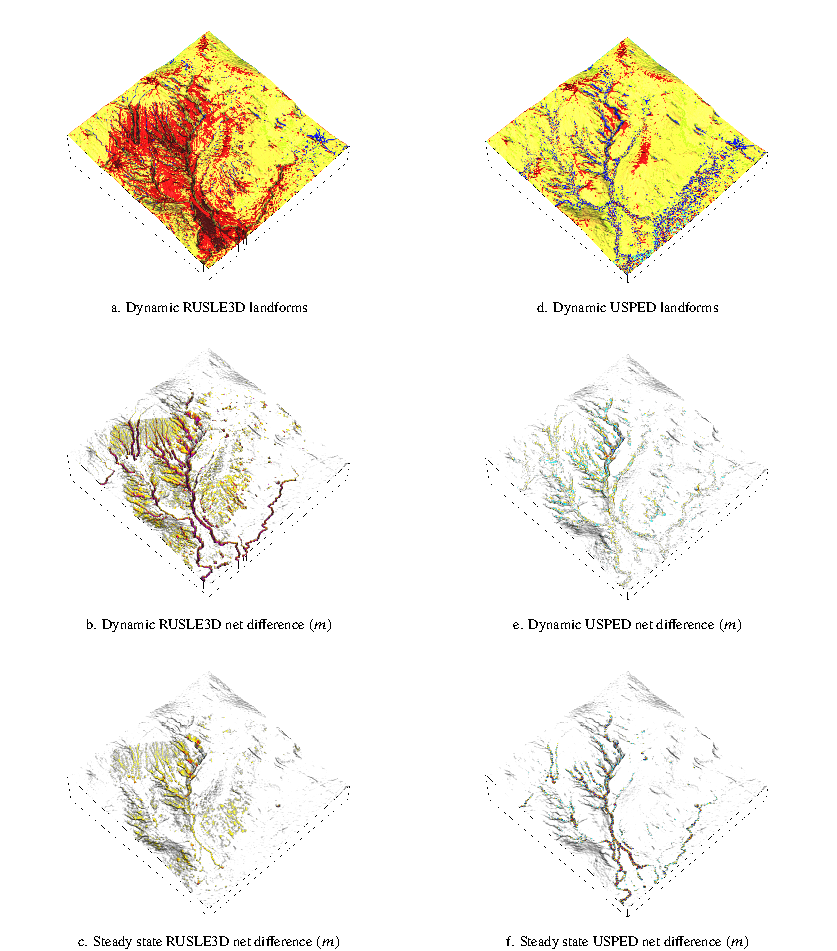
\includegraphics[width=\textwidth,height=0.925\textheight,keepaspectratio]{figures/simulations.pdf}
\caption{Dynamic \DIFaddbeginFL \DIFaddFL{simulations with (a-b) }\DIFaddendFL RUSLE3D and \DIFaddbeginFL \DIFaddFL{(c-d) }\DIFaddendFL USPED
\DIFdelbeginFL \DIFdelFL{simulations
}\DIFdelendFL for a 120~\unit{min} event with a rainfall intensity of 50~\unit{mm~hr}$^{-1}$
\DIFaddbeginFL \DIFaddFL{at 1~}\unit{m} \DIFaddFL{resolution for
Drainage Area 1, Study Subwatershed, Patterson Branch, Fort Bragg, NC.
The (a) net difference }[\unit{m}] \DIFaddFL{and 
(b) landforms for the RUSLE3D simulation.
The (c) net difference }[\unit{m}] \DIFaddFL{and 
(d) landforms for the USPED simulation.
}\DIFaddendFL }
\label{fig:simulations}
\end{figure}

% steady state simwe figure
\begin{figure}
\center
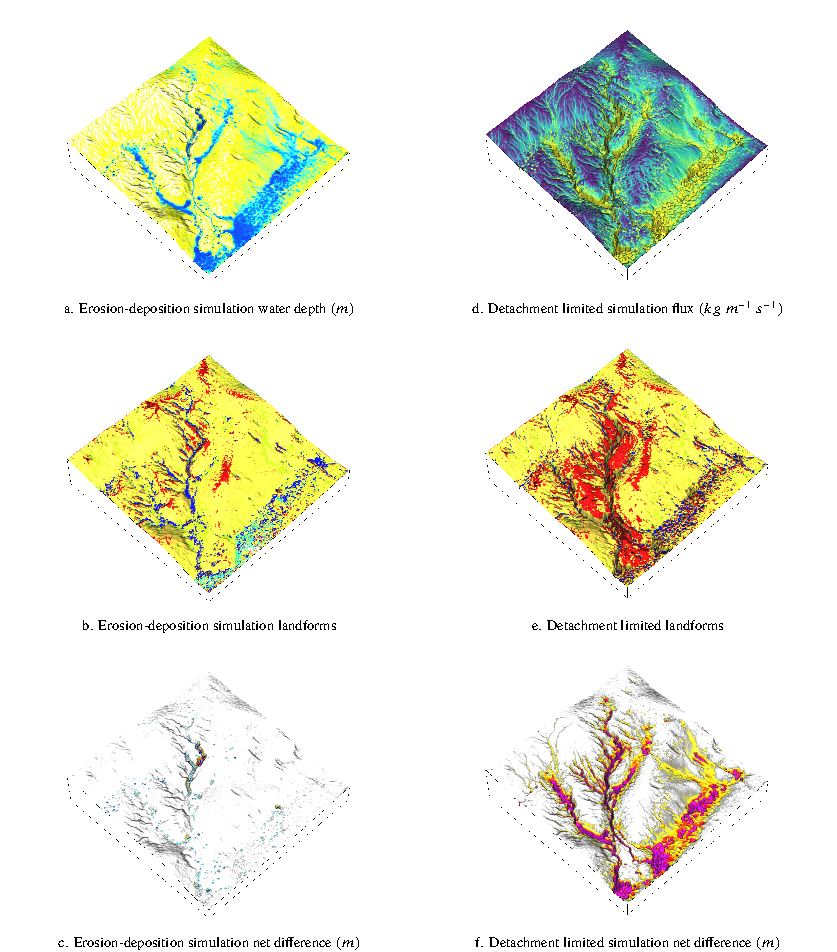
\includegraphics[width=\textwidth,height=0.95\textheight,keepaspectratio]{figures/simwe.pdf}
\caption{\DIFdelbeginFL \DIFdelFL{Steady state }\DIFdelendFL 
\DIFaddbeginFL \DIFaddFL{The (a) net difference }[\unit{m}] \DIFaddFL{and
(b) landforms
simulated with }\DIFaddendFL SIMWE \DIFdelbeginFL \DIFdelFL{simulations
}\DIFdelendFL \DIFaddbeginFL \DIFaddFL{at steady state 
}\DIFaddendFL for \DIFaddbeginFL \DIFaddFL{a }\DIFaddendFL 120~\unit{min} \DIFdelbeginFL \DIFdelFL{events }\DIFdelendFL \DIFaddbeginFL \DIFaddFL{event }\DIFaddendFL with \DIFaddbeginFL \DIFaddFL{a }\DIFaddendFL rainfall \DIFdelbeginFL \DIFdelFL{intensities }\DIFdelendFL \DIFaddbeginFL \DIFaddFL{intensity }\DIFaddendFL of 50~\unit{mm~hr}$^{-1}$
\DIFdelbeginFL \DIFdelFL{and 25}\DIFdelendFL \DIFaddbeginFL \DIFaddFL{at 1}\DIFaddendFL ~\DIFdelbeginFL %DIFDELCMD < \unit{mm~hr}%%%
\DIFdelFL{$^{-1}$}\DIFdelendFL \DIFaddbeginFL \unit{m} \DIFaddFL{resolution for
Drainage Area 1, Study Subwatershed, Patterson Branch, Fort Bragg, NC.
}\DIFaddendFL }
\label{fig:simwe_simulations}
\end{figure}

%DIF >  -------------------- Discussion ---------------------------------
\DIFaddbegin \section{\DIFadd{Discussion}}

%DIF >  limitations
\DIFadd{Limitations of this landscape evolution model include
shallow overland flow, units, computation time, and raster size.
r.sim.terrain only models shallow overland flows, 
not fluvial processes or subsurface flows.
It requires data -- including 
elevation and rainfall intensity -- in metric units. 
The SIMWE model is computationally intensive 
and may require long computation times even with multithreading.
Because SIMWE uses a Green's function Monte Carlo solution 
of the sediment transport equation, 
the accuracy, detail, and smoothness of the results 
depend on the number of random walkers.
While a large number of random walkers will reduce the
numerical error in the path sampling solution,
it will also greatly increase computation time.
A customized compilation of GRASS GIS 
is needed to run SIMWE with more than 7 million random walkers.
This limits the size of rasters 
that can be easily processed with SIMWE,
while RUSLE3D and USPED are much faster, computationally efficient,
and can easily be run on much larger rasters. 
}

%DIF >  future work
\DIFadd{In the future we plan to assess this model
by comparing simulations against 
a monthly timeseries
of submeter resolution surveys
by unmanned aerial systems and terrestrial lidar. 
We also plan to develop a case study demonstrating
how the model can be used as a planning tool 
for landscape restoration. 
Planned enhancements to the model include 
modeling subsurface flows, 
accounting for bedrock, 
and a reverse landscape evolution mode
for backward modeling. 
}

\DIFaddend % -------------------- CONCLUSIONS ---------------------------------
\conclusions

The short-term landscape evolution model 
r.sim.terrain can \DIFdelbegin \DIFdel{realistically }\DIFdelend simulate the development of 
gullies, rills, and hillslopes by overland water erosion
for a range of hydrologic and soil erosion regimes.
The landscape evolution model was tested
with a series of simulations for different 
hydrologic and soil erosion regimes
for a highly eroded sub-watershed on Fort Bragg
with an active gully.
For each regime it generated the 
morphological processes and features expected.
% physics based models
The physics-based SIMWE model 
\DIFdelbegin \DIFdel{realistically simulated short-term topographic change
for steady state hydrologic regimes
at sub-watershed to watershed scales. 
For detachment limited soil erosion regimes
it }\DIFdelend simulated morphological processes 
\DIFdelbegin \DIFdel{including
channel incision, channel widening, and 
the development of knickzones, rills, and scour pits.
For transport limited and }\DIFdelend \DIFaddbegin \DIFadd{for a }\DIFaddend variable erosion-deposition \DIFdelbegin \DIFdel{regimes,
it simulated processes such as 
channel aggradation, }\DIFdelend \DIFaddbegin \DIFadd{regime such as 
gradual aggradation, channel widening, 
}\DIFaddend scouring, and the development of
depositional ridges along the thalweg.
% empirical models
The empirical RUSLE3D \DIFdelbegin \DIFdel{and USPED models
approximated short-term topographic change
at watershed to regional scales. 
For }\DIFdelend \DIFaddbegin \DIFadd{model simulated channel incision
in a }\DIFaddend detachment limited soil erosion \DIFdelbegin \DIFdel{regimes 
RUSLE3D simulated channel incision,
while for transport limited regimes
USPED }\DIFdelend \DIFaddbegin \DIFadd{regime,
while the semi-empirical USPED model
}\DIFaddend simulated channel widening and filling
\DIFaddbegin \DIFadd{in a transport limited regime. 
The elevation change simulated with the USPED model
most closely fit the observed change in the study landscape}\DIFaddend .
% uses & implications
Since \DIFdelbegin \DIFdel{it }\DIFdelend \DIFaddbegin \DIFadd{r.sim.terrain }\DIFaddend is a GIS-based model 
that \DIFdelbegin \DIFdel{realistically }\DIFdelend simulates fine-scale morphological processes and features,
\DIFdelbegin \DIFdel{r.sim.terrain }\DIFdelend \DIFaddbegin \DIFadd{it }\DIFaddend can easily and effectively be used 
in conjunction with other GIS-based tools
for geomorphological research,
land management and conservation,
erosion control, and landscape restoration. 

% --------------------CODE AND DATA------------------------

\DIFdelbegin %DIFDELCMD < \codedataavailability{
%DIFDELCMD < % open science
%DIFDELCMD < As a work of open science
%DIFDELCMD < this study is reproducible, repeatable, and recomputable.
%DIFDELCMD < Since the data, model, GIS, dependencies are all 
%DIFDELCMD < free and open source, the study can easily be reproduced.
%DIFDELCMD < % code
%DIFDELCMD < The landscape evolution model 
%DIFDELCMD < has been implemented in Python as module
%DIFDELCMD < for GRASS GIS, a free and open source GIS.
%DIFDELCMD <  The source code for the model is hosted on GitHub at 
%DIFDELCMD < \url{https://github.com/baharmon/landscape_evolution}
%DIFDELCMD < under the GNU General Public License version 2.
%DIFDELCMD < The code repository also includes Python scripts 
%DIFDELCMD < for running and reproducing the simulations in this paper. 
%DIFDELCMD < The digital object identifier (DOI) 
%DIFDELCMD < for the version of the software documented in this paper is:
%DIFDELCMD < \url{https://doi.org/10.5281/zenodo.2542921}.
%DIFDELCMD < % data
%DIFDELCMD < The geospatial dataset for the study area is available on GitHub at
%DIFDELCMD < \url{https://github.com/baharmon/landscape_evolution_dataset}
%DIFDELCMD < under the 
%DIFDELCMD < \href{https://opendatacommons.org/licenses/odbl/}{Open Database License} 
%DIFDELCMD < with the DOI:
%DIFDELCMD < \url{https://doi.org/10.5281/zenodo.2542929}.
%DIFDELCMD < % osf
%DIFDELCMD < The source code, scripts, data, and results are also hosted
%DIFDELCMD < on the Open Science Framework at 
%DIFDELCMD < \url{https://osf.io/tf6yb/}
%DIFDELCMD < with the DOI:
%DIFDELCMD < \url{https://doi.org/10.17605/osf.io/tf6yb}.
%DIFDELCMD < } 
%DIFDELCMD < %%%
\DIFdelend \DIFaddbegin \codedataavailability{
% open science
As a work of open science
this study is reproducible, repeatable, and recomputable.
Since the data, model, GIS, dependencies are all 
free and open source, the study can easily be reproduced.
% code
The landscape evolution model 
has been implemented in Python as module
for GRASS GIS, a free and open source GIS.
 The source code for the model is hosted on GitHub at 
\url{https://github.com/baharmon/landscape_evolution}
under the GNU General Public License version 2.
The code repository also includes Python scripts 
for running and reproducing the simulations in this paper. 
The digital object identifier (DOI) 
for the version of the software documented in this paper is:
\url{https://doi.org/10.5281/zenodo.2542921}.
There are detailed instructions for running this model in the manual at
\url{https://grass.osgeo.org/grass76/manuals/addons/r.sim.terrain.html}
and the tutorial at
\url{https://github.com/baharmon/landscape_evolution/blob/master/tutorial.md}.
% data
The geospatial dataset for the study area is available on GitHub at
\url{https://github.com/baharmon/landscape_evolution_dataset}
under the 
\href{https://opendatacommons.org/licenses/odbl/}{Open Database License} 
with the DOI:
\url{https://doi.org/10.5281/zenodo.2542929}.
The
\href{https://github.com/baharmon/landscape_evolution_dataset/blob/master/nc_spm_evolution/DATA.md}{data log} has a complete record of the commands used to process the sample data.
% osf
The source code, scripts, data, and results are also hosted
on the Open Science Framework at 
\url{https://osf.io/tf6yb/}
with the DOI:
\url{https://doi.org/10.17605/osf.io/tf6yb}.
}
\DIFaddend 

% ----------------------------------------------------------------------------

\noappendix 

\authorcontribution{
Brendan Harmon developed 
the models, code, data, case studies, and manuscript.
Helena Mitasova contributed to the development 
of the models and case studies and revised the manuscript.
Anna Petrasova and Vaclav Petras
contributed to the development of the code.
All authors read and approved the final manuscript.
}

\competinginterests{The authors declare that they have no conflict of interest.} 

\begin{acknowledgements}
We acknowledge the GRASS GIS Development Community
for developing and maintaining GRASS GIS.
\end{acknowledgements}

% ---------------------REFERENCES---------------------------
\bibliographystyle{copernicus}
\bibliography{landscape_evolution.bib}

\end{document}
